% ============================================================================
% Healthcare Data Warehouse & Analytics Platform - Developer Guide
% A Beginner-Friendly, Step-by-Step Technical Documentation
% Version 1.0 - Enhanced Educational Edition
% ============================================================================
\documentclass[12pt, a4paper, oneside]{report}

% --- Packages ---------------------------------------------------------------
\usepackage[utf8]{inputenc}
\usepackage[T1]{fontenc}
\usepackage{lmodern}
\usepackage[margin=2.5cm]{geometry}
\usepackage{graphicx}
\usepackage{xcolor}
\usepackage{listings}
\usepackage{hyperref}
\usepackage{booktabs}
\usepackage{longtable}
\usepackage{tabularx}
\usepackage{array}
\usepackage{enumitem}
\usepackage{tikz}
\usetikzlibrary{shapes.geometric, arrows.meta, positioning, fit, calc, backgrounds, decorations.pathreplacing, shadows}
\usepackage{fancyhdr}
\usepackage{titlesec}
\usepackage{tcolorbox}
\tcbuselibrary{skins, breakable, listings}
\usepackage{fontawesome5}
\usepackage{float}
\usepackage{caption}
\usepackage{subcaption}
\usepackage{pifont}
\usepackage{amssymb}
\usepackage{amsmath}
\usepackage{setspace}
\usepackage{makeidx}

\makeindex

% --- Color Definitions ------------------------------------------------------
\definecolor{primary}{HTML}{1B4F72}
\definecolor{secondary}{HTML}{2E86C1}
\definecolor{accent}{HTML}{E74C3C}
\definecolor{success}{HTML}{27AE60}
\definecolor{warning}{HTML}{F39C12}
\definecolor{codebackground}{HTML}{F7F9FC}
\definecolor{codeborder}{HTML}{D5E8F0}
\definecolor{keywordcolor}{HTML}{8E44AD}
\definecolor{stringcolor}{HTML}{27AE60}
\definecolor{commentcolor}{HTML}{7F8C8D}
\definecolor{bronzecolor}{HTML}{CD7F32}
\definecolor{silvercolor}{HTML}{808080}
\definecolor{goldcolor}{HTML}{DAA520}
\definecolor{tipbg}{HTML}{E8F8F5}
\definecolor{warnbg}{HTML}{FEF9E7}
\definecolor{notebg}{HTML}{EBF5FB}
\definecolor{importantbg}{HTML}{FDEDEC}
\definecolor{objectivebg}{HTML}{EBF5FB}
\definecolor{summarybg}{HTML}{E8F8F5}
\definecolor{exercisebg}{HTML}{FEF9E7}

% --- Hyperref Setup ---------------------------------------------------------
\hypersetup{
    colorlinks=true,
    linkcolor=primary,
    urlcolor=secondary,
    citecolor=primary,
    pdfauthor={Mahmoud Salem},
    pdftitle={Healthcare Data Warehouse - Developer Guide v2.0},
    pdfsubject={Data Engineering Documentation},
}

% --- Listings Setup ---------------------------------------------------------
\lstdefinestyle{basestyle}{
    backgroundcolor=\color{codebackground},
    basicstyle=\ttfamily\small,
    breakatwhitespace=false,
    breaklines=true,
    captionpos=b,
    keepspaces=true,
    showspaces=false,
    showstringspaces=false,
    showtabs=false,
    tabsize=2,
    frame=single,
    rulecolor=\color{codeborder},
    framesep=5pt,
    xleftmargin=10pt,
    xrightmargin=5pt,
    aboveskip=10pt,
    belowskip=8pt,
}

\lstdefinestyle{pythonstyle}{
    style=basestyle,
    language=Python,
    keywordstyle=\color{keywordcolor}\bfseries,
    stringstyle=\color{stringcolor},
    commentstyle=\color{commentcolor}\itshape,
    morekeywords={self, True, False, None, as, with, yield, async, await},
}

\lstdefinestyle{sqlstyle}{
    style=basestyle,
    language=SQL,
    keywordstyle=\color{keywordcolor}\bfseries,
    stringstyle=\color{stringcolor},
    commentstyle=\color{commentcolor}\itshape,
    morekeywords={NVARCHAR, BIGINT, BIT, UNIQUEIDENTIFIER, DATETIME2, DECIMAL,
                  INT, VARCHAR, DATE, FLOAT, TINYINT, HASH, REPLICATE, CLUSTERED,
                  COLUMNSTORE, PARTITION, DISTRIBUTION},
}

\lstdefinestyle{yamlstyle}{
    style=basestyle,
    keywordstyle=\color{keywordcolor}\bfseries,
    stringstyle=\color{stringcolor},
    commentstyle=\color{commentcolor}\itshape,
    morecomment=[l]{\#},
    morestring=[b]",
    morestring=[b]',
}

\lstdefinestyle{bashstyle}{
    style=basestyle,
    language=bash,
    keywordstyle=\color{keywordcolor}\bfseries,
    stringstyle=\color{stringcolor},
    commentstyle=\color{commentcolor}\itshape,
}

\lstdefinestyle{dockerstyle}{
    style=basestyle,
    keywordstyle=\color{keywordcolor}\bfseries,
    morekeywords={FROM, RUN, COPY, WORKDIR, EXPOSE, CMD, ENV, ARG,
                  ENTRYPOINT, ADD, VOLUME, LABEL, HEALTHCHECK},
    stringstyle=\color{stringcolor},
    commentstyle=\color{commentcolor}\itshape,
    morecomment=[l]{\#},
}

% --- Custom tcolorbox environments -----------------------------------------
\newtcolorbox{tipbox}[1][]{
    enhanced, breakable,
    colback=tipbg, colframe=success,
    fonttitle=\bfseries,
    title={\faLightbulb\ Tip},
    left=6pt, right=6pt, top=4pt, bottom=4pt,
    #1
}

\newtcolorbox{warningbox}[1][]{
    enhanced, breakable,
    colback=warnbg, colframe=warning,
    fonttitle=\bfseries,
    title={\faExclamationTriangle\ Warning},
    left=6pt, right=6pt, top=4pt, bottom=4pt,
    #1
}

\newtcolorbox{notebox}[1][]{
    enhanced, breakable,
    colback=notebg, colframe=secondary,
    fonttitle=\bfseries,
    title={\faInfoCircle\ Note},
    left=6pt, right=6pt, top=4pt, bottom=4pt,
    #1
}

\newtcolorbox{importantbox}[1][]{
    enhanced, breakable,
    colback=importantbg, colframe=accent,
    fonttitle=\bfseries,
    title={\faExclamationCircle\ Important},
    left=6pt, right=6pt, top=4pt, bottom=4pt,
    #1
}

\newtcolorbox{conceptbox}[2][]{
    enhanced, breakable,
    colback=white, colframe=primary,
    fonttitle=\bfseries\large,
    title={#2},
    left=8pt, right=8pt, top=6pt, bottom=6pt,
    #1
}

\newtcolorbox{objectivebox}[1][]{
    enhanced, breakable,
    colback=objectivebg, colframe=primary,
    fonttitle=\bfseries,
    title={\faBookmark\ Learning Objectives},
    left=6pt, right=6pt, top=4pt, bottom=4pt,
    #1
}

\newtcolorbox{summarybox}[1][]{
    enhanced, breakable,
    colback=summarybg, colframe=success,
    fonttitle=\bfseries,
    title={\faCheckCircle\ Chapter Summary},
    left=6pt, right=6pt, top=4pt, bottom=4pt,
    #1
}

\newtcolorbox{exercisebox}[1][]{
    enhanced, breakable,
    colback=exercisebg, colframe=warning,
    fonttitle=\bfseries,
    title={\faPen\ Try It Yourself},
    left=6pt, right=6pt, top=4pt, bottom=4pt,
    #1
}

% --- Header and Footer ------------------------------------------------------
\pagestyle{fancy}
\fancyhf{}
\fancyhead[L]{\small\textcolor{primary}{\nouppercase{\leftmark}}}
\fancyhead[R]{\small\textcolor{primary}{Healthcare DW \& Analytics}}
\fancyfoot[L]{\scriptsize Prepared by Mahmoud Salem\\\textcolor{secondary}{\url{linkedin.com/in/ma7moudalysalem}}}
\fancyfoot[C]{}
\fancyfoot[R]{\thepage}
\renewcommand{\headrulewidth}{0.4pt}
\renewcommand{\footrulewidth}{0.2pt}

% --- Title Formatting -------------------------------------------------------
\titleformat{\chapter}[display]
    {\normalfont\huge\bfseries\color{primary}}
    {\chaptertitlename\ \thechapter}{20pt}{\Huge}
\titlespacing*{\chapter}{0pt}{-20pt}{30pt}

\titleformat{\section}
    {\normalfont\Large\bfseries\color{primary}}
    {\thesection}{1em}{}

\titleformat{\subsection}
    {\normalfont\large\bfseries\color{secondary}}
    {\thesubsection}{1em}{}

% --- Line Spacing -----------------------------------------------------------
\setstretch{1.25}

% ============================================================================
% DOCUMENT BEGINS
% ============================================================================
\begin{document}

% --- Title Page -------------------------------------------------------------
\begin{titlepage}
    \centering
    \vspace*{2cm}

    {\Huge\bfseries\color{primary} Healthcare Data Warehouse\\[0.3cm]
     \& Analytics Platform}\\[1cm]

    {\LARGE\color{secondary} Developer Guide}\\[0.5cm]

    {\large\color{primary} A Beginner-Friendly, Step-by-Step Technical Documentation}\\[0.3cm]
    {\normalsize\color{secondary} Version 1.0}\\[2cm]

    
\begin{tikzpicture}[
        node distance=0.8cm,
        every node/.style={font=\small},
        box/.style={rectangle, rounded corners=5pt, minimum width=3cm,
                    minimum height=0.8cm, text=white, font=\small\bfseries,
                    drop shadow}
    ]
        \node[box, fill=bronzecolor] (bronze) {Bronze Layer};
        \node[box, fill=silvercolor, right=of bronze] (silver) {Silver Layer};
        \node[box, fill=goldcolor, right=of silver] (gold) {Gold Layer};

        \draw[-{Stealth[length=3mm]}, thick, color=primary]
            (bronze) -- (silver);
        \draw[-{Stealth[length=3mm]}, thick, color=primary]
            (silver) -- (gold);
    \end{tikzpicture}

    \vfill

    {\large\textbf{Digital Egypt Pioneers Initiative (DEPI)}\\
     AI \& Data Science Track --- Microsoft Data Engineer}\\[1.5cm]

    \rule{0.4\textwidth}{0.4pt}\\[0.8cm]
    {\small\itshape Prepared by}\\[0.3cm]
    {\Large\bfseries Mahmoud Salem}\\[0.2cm]
    {\small\color{secondary}\url{https://linkedin.com/in/ma7moudalysalem}}\\[1cm]

    {\small Version 1.0 --- \today}
\end{titlepage}

% --- Table of Contents ------------------------------------------------------
\tableofcontents
\newpage

% --- List of Figures --------------------------------------------------------
\listoffigures
\newpage


% ============================================================================
% CHAPTER 1: INTRODUCTION
% ============================================================================
\chapter{Introduction}
\label{ch:introduction}

\begin{objectivebox}
By the end of this chapter, you will be able to:
\begin{itemize}
    \item Explain what a data warehouse is and how it differs from an operational database
    \item Describe the purpose and scope of this project
    \item Identify all the technologies used and what role each one plays
    \item Understand the difference between OLTP and OLAP systems
\end{itemize}
\end{objectivebox}

\section{What Is This Project?}

Imagine a hospital network with \textbf{5 hospitals and 20+ clinics} spread across Egypt. Every day, thousands of patients visit these facilities. Their data --- medical records, lab results, insurance claims, vital signs --- is scattered across many different computer systems that do not talk to each other.

This is a common real-world problem called \textbf{data silos}: each system stores its own data in its own format, making it nearly impossible to get a complete picture of what is happening across the entire network.

This project builds a \textbf{centralized data warehouse} that:
\begin{enumerate}[label=\textcolor{primary}{\arabic*.}]
    \item \textbf{Collects} all that scattered data into one place
    \item \textbf{Cleans and organizes} it so it is consistent and reliable
    \item \textbf{Transforms} it into a format optimized for analytics
    \item \textbf{Presents} it through interactive dashboards for decision-makers
    \item \textbf{Monitors} real-time vital signs and raises alerts for anomalies
\end{enumerate}

\begin{conceptbox}{What Is a Data Warehouse?}
A \textbf{data warehouse}\index{Data Warehouse} is a special database designed for \textit{analyzing} data, not for running daily operations. Think of it this way:

\begin{itemize}
    \item \textbf{OLTP (Operational Database)}\index{OLTP} = The cash register at a store. It handles individual transactions quickly: ``Patient X visited Doctor Y on this date.''
    \item \textbf{OLAP (Data Warehouse)}\index{OLAP} = The accountant's summary report. It answers big-picture questions: ``How many patients were readmitted within 30 days across all hospitals this quarter?''
\end{itemize}

Here is a simple comparison to make this concrete:

\begin{center}
\small
\begin{tabular}{p{3.5cm} p{5cm} p{5cm}}
    \toprule
    \textbf{Aspect} & \textbf{OLTP (Cash Register)} & \textbf{OLAP (Accountant)} \\
    \midrule
    Typical query & ``Get patient \#123's record'' & ``Average cost per diagnosis across all hospitals'' \\
    Speed priority & Fast writes (milliseconds) & Fast reads over millions of rows \\
    Data scope & Current data & Historical data (months/years) \\
    Users & Doctors, nurses, apps & Analysts, managers, dashboards \\
    \bottomrule
\end{tabular}
\end{center}
\end{conceptbox}

\section{Who Is This Guide For?}

This guide is written for \textbf{students and junior developers} who are:
\begin{itemize}
    \item Learning data engineering for the first time
    \item Familiar with basic programming (Python, SQL) but new to cloud and big data
    \item Joining this project or building something similar
\end{itemize}

We explain \textbf{every concept before showing you the code}, so you always understand \textit{why} before \textit{how}. No prior knowledge of cloud computing, data warehousing, or healthcare IT is assumed.

\section{Technologies at a Glance}

Before diving in, here is every technology we use and \textit{what it does} in plain English:

\begin{longtable}{>{\bfseries}p{3.5cm} p{4cm} p{6cm}}
    \toprule
    \textbf{Technology} & \textbf{Category} & \textbf{What It Does (Simply)} \\
    \midrule
    \endhead
    Python 3.11 & Language & The main programming language for scripts and data processing \\
    T-SQL & Language & Microsoft's flavor of SQL for querying databases \\
    PySpark & Language & Python + Apache Spark for processing huge datasets \\
    DAX & Language & Formula language for Power BI calculations \\
    \midrule
    SQL Server 2022 & Database & Stores raw patient data locally (like a local filing cabinet) \\
    Azure Synapse & Database & Cloud data warehouse for analytics (the big filing room) \\
    \midrule
    Azure Data Lake & Storage & Stores files (CSV, JSON, Parquet) in the cloud cheaply \\
    Azure Data Factory & Orchestration & Moves data between systems on a schedule (like a delivery truck) \\
    Azure Databricks & Processing & Runs Spark jobs to clean and transform data (the factory) \\
    Azure Event Hubs & Streaming & Receives real-time data streams (like a mail slot) \\
    \midrule
    Docker & DevOps & Packages software into containers for consistent environments \\
    GitHub Actions & DevOps & Automatically tests code every time you push changes \\
    Git & DevOps & Version control --- tracks all changes to your code \\
    \midrule
    Power BI & Visualization & Creates interactive business dashboards \\
    Streamlit & Visualization & Python framework for building simple web dashboards \\
    \midrule
    Synthea & Data Generation & Generates realistic (but fake) patient medical records \\
    Faker & Data Generation & Python library for generating fake data (names, dates, etc.) \\
    \bottomrule
\end{longtable}

\begin{tipbox}
    Do not worry about memorizing all these technologies now. Each chapter introduces the relevant tools \textit{when you need them}. This table is here as a reference you can come back to at any time.
\end{tipbox}

\section{How to Read This Guide}

This guide is structured to be read \textbf{in order}, with each chapter building on the previous one. However, if you already know a topic, feel free to skip ahead. Here is the recommended path:

\begin{enumerate}[label=\textcolor{primary}{\textbf{\arabic*.}}]
    \item \textbf{Chapters 1--2:} Understand the project scope and folder structure
    \item \textbf{Chapters 3--4:} Learn the architecture and data model (the ``blueprint'')
    \item \textbf{Chapter 5:} Understand where our data comes from
    \item \textbf{Chapters 6--8:} Development environment (Docker, config, CI/CD)
    \item \textbf{Chapters 9--10:} Testing and Git workflow
    \item \textbf{Chapters 11--12:} SQL analytics and Azure cloud services
    \item \textbf{Chapters 13--15:} Getting started, milestones, and team guidelines
    \item \textbf{Chapter 16:} Conclusion and your learning roadmap
    \item \textbf{Glossary:} Quick-reference for any unfamiliar terms
\end{enumerate}

\begin{summarybox}
\textbf{Key Takeaways:}
\begin{itemize}
    \item This project builds a centralized data warehouse for a hospital network using Azure cloud services
    \item A data warehouse (OLAP) is optimized for analytics, unlike operational databases (OLTP) which handle daily transactions
    \item The project uses Python, SQL, PySpark, Docker, Azure services, and Power BI
    \item This guide explains every concept from first principles --- no prior cloud or data warehousing experience needed
\end{itemize}
\end{summarybox}


% ============================================================================
% CHAPTER 2: PROJECT STRUCTURE
% ============================================================================
\chapter{Project Structure --- Every Folder Explained}
\label{ch:structure}

\begin{objectivebox}
By the end of this chapter, you will be able to:
\begin{itemize}
    \item Navigate the project directory with confidence
    \item Explain the purpose of every folder and root-level file
    \item Understand Python package conventions (\texttt{\_\_init\_\_.py})
    \item Know which files are tracked by Git and which are ignored
\end{itemize}
\end{objectivebox}

When you first open this project, you will see many folders and files. Do not worry --- each one has a clear purpose. Let us go through \textbf{every single one}.

\section{The Big Picture}

\begin{lstlisting}[style=bashstyle, caption={Complete project directory tree}]
healthcare-data-warehouse/
|-- src/                    # All Python source code
|   |-- generators/         # Scripts that create fake data
|   +-- synthea/            # Synthea config files
|-- notebooks/              # Jupyter and Databricks notebooks
|-- sql/                    # All SQL scripts
|   |-- ddl/                # CREATE TABLE statements
|   |-- queries/            # Analytical queries
|   +-- stored_procedures/  # Reusable SQL procedures
|-- pipelines/
|   +-- adf_templates/      # Azure Data Factory templates
|-- dashboards/             # Power BI files and screenshots
|   +-- screenshots/        # Dashboard images
|-- docs/                   # Documentation
|   |-- architecture/       # Architecture diagrams
|   +-- data_dictionary/    # Column-level documentation
|-- tests/                  # Automated test files
|-- docker/                 # Docker configuration
|-- data/                   # Data files (NOT in git)
|   |-- raw/                # Raw CSV/JSON files
|   |-- cleaned/            # Cleaned Parquet files
|   +-- gold/               # Final analytics-ready files
|-- config/                 # App configuration files
|-- .github/workflows/      # CI/CD pipeline config
|-- requirements.txt        # Python dependencies
|-- .env.example            # Environment variable template
|-- setup.cfg               # Linting and test config
|-- docker-compose.yml      # (inside docker/)
+-- README.md               # Project overview
\end{lstlisting}

\begin{notebox}
    The tree above uses a common convention: \texttt{|--} means ``this item is inside the folder above it,'' and \texttt{+--} means ``this is the last item in that folder.'' Lines with \texttt{\#} are comments explaining what each folder contains.
\end{notebox}

\section{Folder-by-Folder Breakdown}

\subsection{src/ --- The Source Code}

This is where all the Python code lives. It has two subfolders:

\begin{itemize}
    \item \texttt{src/generators/} --- Contains Python scripts that \textbf{generate fake healthcare data}:
    \begin{itemize}
        \item \texttt{generate\_claims.py} --- Creates 200,000 fake insurance claims
        \item \texttt{simulate\_vitals.py} --- Simulates IoT vital sign readings in real-time
        \item \texttt{provider\_api.py} --- A Flask web API that serves doctor/provider data
    \end{itemize}
    \item \texttt{src/synthea/} --- Configuration for \textbf{Synthea}\index{Synthea}, a tool that generates realistic patient records
\end{itemize}

\begin{tipbox}
    Every Python package (folder) has an \texttt{\_\_init\_\_.py} file. This is a Python convention that tells Python: ``This folder is a package, you can import from it.'' Even if the file is empty, it must exist. Without it, Python cannot use \texttt{import} statements to load code from that folder.
\end{tipbox}

\subsection{notebooks/ --- Jupyter and Databricks Notebooks}

Notebooks combine code, output, and explanations in one document. We use them for:
\begin{itemize}
    \item \textbf{Exploratory Data Analysis (EDA)}\index{EDA} --- Analyzing the generated data with charts and statistics
    \item \textbf{Databricks PySpark notebooks} --- Running Spark transformations in the cloud
\end{itemize}

\begin{conceptbox}{What Is a Jupyter Notebook?}
A \textbf{Jupyter Notebook}\index{Jupyter Notebook} is an interactive document that contains:
\begin{itemize}
    \item \textbf{Code cells} --- blocks of Python code you can run one at a time
    \item \textbf{Output cells} --- the results (tables, charts, text) appear directly below the code
    \item \textbf{Markdown cells} --- formatted text for explanations and documentation
\end{itemize}
Think of it as a lab notebook where you can write notes \textit{and} run experiments in the same document. Files end with \texttt{.ipynb} (short for ``Interactive Python Notebook'').
\end{conceptbox}

\subsection{sql/ --- All SQL Scripts}

\begin{itemize}
    \item \texttt{sql/ddl/} --- \textbf{DDL}\index{DDL} stands for ``Data Definition Language.'' These are \texttt{CREATE TABLE} statements that define the structure of our tables --- columns, data types, constraints, indexes.
    \item \texttt{sql/queries/} --- 10+ analytical queries that answer business questions (e.g., ``What is the 30-day readmission rate?'')
    \item \texttt{sql/stored\_procedures/} --- Reusable SQL code blocks stored inside the database
\end{itemize}

\begin{conceptbox}{DDL vs DML --- What Is the Difference?}
\begin{itemize}
    \item \textbf{DDL (Data Definition Language):}\index{DDL} Commands that \textit{define structure} --- \texttt{CREATE TABLE}, \texttt{ALTER TABLE}, \texttt{DROP TABLE}
    \item \textbf{DML (Data Manipulation Language):}\index{DML} Commands that \textit{work with data} --- \texttt{SELECT}, \texttt{INSERT}, \texttt{UPDATE}, \texttt{DELETE}
\end{itemize}
Think of DDL as building the shelves, and DML as putting books on those shelves.

\textbf{Simple example:}
\begin{lstlisting}[style=sqlstyle]
-- DDL: Build the shelf
CREATE TABLE patients (
    patient_id INT PRIMARY KEY,
    name VARCHAR(100)
);

-- DML: Put books on the shelf
INSERT INTO patients VALUES (1, 'Ahmed Ali');
SELECT * FROM patients;
\end{lstlisting}
\end{conceptbox}

\subsection{pipelines/ --- Data Pipeline Templates}

Contains Azure Data Factory (ADF)\index{Azure Data Factory} ARM templates --- these are JSON files that define automated data movement workflows. Think of them as ``recipes'' that tell Azure: ``Every day at 2 AM, copy new files from the Data Lake into Databricks for processing.''

\subsection{dashboards/ --- Visualization Files}

\begin{itemize}
    \item Power BI \texttt{.pbix} files (the actual dashboards)
    \item Streamlit Python app (optional web-based dashboard)
    \item Screenshots of the dashboards
\end{itemize}

\subsection{docs/ --- Documentation}

\begin{itemize}
    \item \texttt{docs/architecture/} --- Visual diagrams showing how data flows through the system
    \item \texttt{docs/data\_dictionary/} --- Detailed description of every column in every table
\end{itemize}

\subsection{tests/ --- Automated Tests}

Contains \texttt{pytest}\index{pytest} test files that verify the project is set up correctly. We explain these in detail in Chapter~\ref{ch:testing}.

\subsection{docker/ --- Container Configuration}

Contains files that let you run the entire development environment in Docker containers. More on this in Chapter~\ref{ch:docker}.

\subsection{data/ --- Data Files (Git-Ignored)}

This folder holds actual data files, but they are \textbf{not tracked by Git} because:
\begin{itemize}
    \item Data files can be \textbf{very large} (gigabytes)
    \item They can be \textbf{regenerated} by running the generator scripts
    \item They might contain \textbf{sensitive information} in real projects
\end{itemize}

The three subfolders correspond to the \textbf{Medallion Architecture}\index{Medallion Architecture} layers (explained in Chapter~\ref{ch:architecture}).

\section{Root-Level Files Explained}

\begin{longtable}{>{\ttfamily\small}p{4.5cm} p{9cm}}
    \toprule
    \normalfont\textbf{File} & \textbf{Purpose} \\
    \midrule
    \endhead
    README.md & The ``front page'' of the project on GitHub. Written in Markdown. \\
    requirements.txt & Lists all Python packages the project needs. \\
    .env.example & A template showing what environment variables to set. \\
    .gitignore & Tells Git which files to NOT track (data, secrets, caches). \\
    .gitattributes & Ensures consistent line endings across Windows/Mac/Linux. \\
    setup.cfg & Configuration for code linting (flake8) and testing (pytest). \\
    \bottomrule
\end{longtable}

\begin{exercisebox}
\textbf{Practice:} Open the project in your file explorer or terminal and:
\begin{enumerate}
    \item List all files in the \texttt{src/generators/} folder. How many Python files are there?
    \item Open \texttt{.gitignore} and find which file patterns are ignored. Why is \texttt{.env} ignored but \texttt{.env.example} is not?
    \item Look at the \texttt{data/} folder. Is it empty? Why does it exist in Git even though its contents are ignored? \textit{(Hint: look for \texttt{.gitkeep} files)}
\end{enumerate}
\end{exercisebox}

\begin{summarybox}
\textbf{Key Takeaways:}
\begin{itemize}
    \item The project follows a clean, modular folder structure separating code (\texttt{src/}), data (\texttt{data/}), tests (\texttt{tests/}), docs (\texttt{docs/}), and config files
    \item Each Python package folder contains an \texttt{\_\_init\_\_.py} file
    \item Data files and secrets (\texttt{.env}) are excluded from Git using \texttt{.gitignore}
    \item The \texttt{data/} subfolders (raw, cleaned, gold) mirror the Medallion Architecture layers
\end{itemize}
\end{summarybox}


% ============================================================================
% CHAPTER 3: ARCHITECTURE
% ============================================================================
\chapter{The Architecture --- How Data Flows}
\label{ch:architecture}

\begin{objectivebox}
By the end of this chapter, you will be able to:
\begin{itemize}
    \item Explain the Medallion Architecture and why it uses three layers
    \item Describe what happens at each layer (Bronze, Silver, Gold)
    \item Trace the complete data flow from source to dashboard (both batch and streaming)
    \item Understand the difference between batch and streaming data processing
    \item Define key terms: Delta Lake, ACID transactions, schema enforcement
\end{itemize}
\end{objectivebox}

\section{The Medallion Architecture}

Our project uses the \textbf{Medallion Architecture}\index{Medallion Architecture}, a popular pattern in modern data engineering. It organizes data into three layers, each progressively cleaner and more useful:

\begin{figure}[H]
\centering
\resizebox{\textwidth}{!}{%
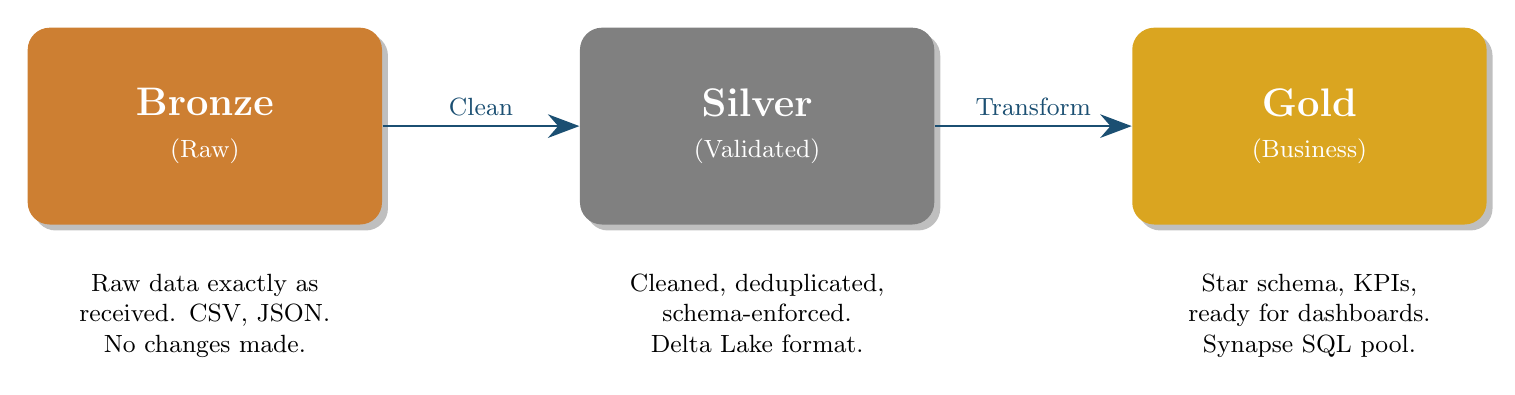
\begin{tikzpicture}[
    node distance=2cm,
    layer/.style={rectangle, rounded corners=8pt, minimum width=4.5cm,
                  minimum height=2.5cm, text=white, font=\bfseries,
                  align=center, drop shadow},
    arrow/.style={-{Stealth[length=4mm]}, thick, color=primary},
    desc/.style={font=\small, text width=4.2cm, align=center}
]

% Layers
\node[layer, fill=bronzecolor] (bronze) {
    \Large Bronze\\[3pt]
    \normalfont\small (Raw)
};
\node[layer, fill=silvercolor, right=2.5cm of bronze] (silver) {
    \Large Silver\\[3pt]
    \normalfont\small (Validated)
};
\node[layer, fill=goldcolor, right=2.5cm of silver] (gold) {
    \Large Gold\\[3pt]
    \normalfont\small (Business)
};

% Arrows
\draw[arrow] (bronze) -- node[above, font=\small\color{primary}] {Clean} (silver);
\draw[arrow] (silver) -- node[above, font=\small\color{primary}] {Transform} (gold);

% Descriptions below
\node[desc, below=0.5cm of bronze] {
    Raw data exactly as\\received. CSV, JSON.\\No changes made.
};
\node[desc, below=0.5cm of silver] {
    Cleaned, deduplicated,\\schema-enforced.\\Delta Lake format.
};
\node[desc, below=0.5cm of gold] {
    Star schema, KPIs,\\ready for dashboards.\\Synapse SQL pool.
};

\end{tikzpicture}%
}
\caption{The Medallion Architecture: Bronze $\rightarrow$ Silver $\rightarrow$ Gold}
\label{fig:medallion}
\end{figure}

\begin{conceptbox}{Why Three Layers?}
Think of it like cooking:
\begin{enumerate}[label=\textcolor{primary}{\arabic*.}]
    \item \textbf{Bronze} = Raw ingredients from the market (unwashed vegetables, uncut meat). You store them as-is so you always have the original.
    \item \textbf{Silver} = Washed, peeled, and sliced ingredients. Clean and ready to combine, but not yet a dish.
    \item \textbf{Gold} = The finished meal, plated and ready to serve. This is what the business consumers (dashboards, analysts) eat.
\end{enumerate}
Why not just go straight from raw to final? Because if you make a mistake in cooking, you can go back to the cleaned ingredients (Silver) instead of starting from the raw market produce (Bronze) all over again. Each layer acts as a \textbf{checkpoint} you can return to.
\end{conceptbox}

\subsection{Bronze Layer --- Raw Data Landing}

\begin{itemize}
    \item \textbf{What goes here:} Raw CSV files from Synthea, JSON from the claims generator, streaming data from IoT sensors
    \item \textbf{Where it lives:} Azure Data Lake Gen2, container named \texttt{bronze}
    \item \textbf{Rule:} \textit{Never modify data in Bronze.} It is your backup, your ``single source of truth''
    \item \textbf{Data formats:} CSV, JSON, raw Parquet
\end{itemize}

\begin{warningbox}
    The Bronze layer is \textbf{immutable} (read-only after writing). This is critical because if a bug in your cleaning code corrupts the Silver layer, you can always re-process from Bronze. Treat Bronze like a backup tape --- write once, read many times, never edit.
\end{warningbox}

\subsection{Silver Layer --- Cleaned and Validated}

\begin{itemize}
    \item \textbf{What happens here:}
    \begin{itemize}
        \item Remove duplicate records
        \item Handle missing values (nulls)
        \item Enforce correct data types (dates are dates, numbers are numbers)
        \item Normalize formats (all dates become ISO 8601: \texttt{YYYY-MM-DD})
        \item Standardize drug names using RxNorm codes
    \end{itemize}
    \item \textbf{Where it lives:} Databricks Delta Lake tables, container named \texttt{silver}
    \item \textbf{Data format:} Delta Lake (Parquet + transaction log)
\end{itemize}

\begin{conceptbox}{What Is Delta Lake?}
\textbf{Delta Lake}\index{Delta Lake} is a storage format built on top of Parquet files. It adds:
\begin{itemize}
    \item \textbf{ACID Transactions}\index{ACID} --- your writes either fully succeed or fully fail, never half-done
    \item \textbf{Schema Enforcement} --- rejects data that does not match the expected columns/types
    \item \textbf{Time Travel} --- you can query data as it looked yesterday or last week
    \item \textbf{Versioning} --- every change creates a new version you can roll back to
\end{itemize}
Think of it as ``Excel with an undo history that never loses anything.''

\textbf{Simple example of Time Travel:}
\begin{lstlisting}[style=sqlstyle]
-- Query the current version of the table
SELECT * FROM silver.patients;

-- Query the table as it was 3 versions ago
SELECT * FROM silver.patients VERSION AS OF 3;

-- Query the table as it was yesterday
SELECT * FROM silver.patients TIMESTAMP AS OF '2024-01-15';
\end{lstlisting}
\end{conceptbox}

\subsection{Gold Layer --- Business-Ready}

\begin{itemize}
    \item \textbf{What happens here:} Data is reorganized into a \textbf{Star Schema}\index{Star Schema} (explained in Chapter~\ref{ch:datamodel}) with pre-calculated metrics
    \item \textbf{Where it lives:} Azure Synapse Analytics dedicated SQL pool
    \item \textbf{Who uses it:} Power BI dashboards, analysts writing SQL queries, Streamlit apps
\end{itemize}

\section{The Complete Data Flow}

Now that you understand the three layers, let us see how data actually moves through the system. There are two paths: \textbf{batch} (scheduled, large volumes) and \textbf{streaming} (real-time, continuous).

\begin{figure}[H]
\centering
\resizebox{\textwidth}{!}{%
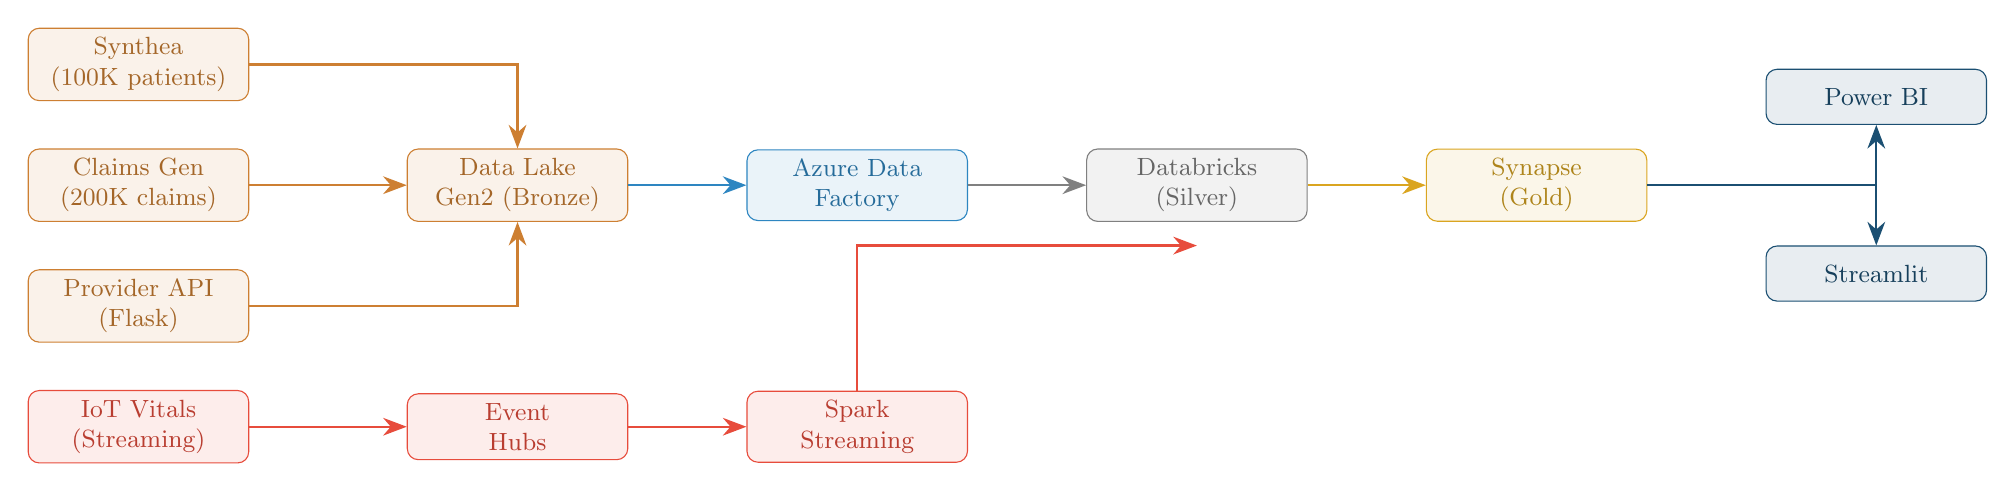
\begin{tikzpicture}[
    node distance=0.6cm and 1.2cm,
    box/.style={rectangle, rounded corners=4pt, minimum width=2.8cm,
                minimum height=0.7cm, draw=#1, fill=#1!10,
                font=\small, align=center, text=#1!80!black},
    arrow/.style={-{Stealth[length=3mm]}, thick, color=#1},
    label/.style={font=\tiny\itshape, color=gray}
]

% Data Sources
\node[box=bronzecolor] (synthea) {Synthea\\(100K patients)};
\node[box=bronzecolor, below=of synthea] (claims) {Claims Gen\\(200K claims)};
\node[box=bronzecolor, below=of claims] (api) {Provider API\\(Flask)};
\node[box=accent, below=of api] (iot) {IoT Vitals\\(Streaming)};

% Bronze
\node[box=bronzecolor, right=2cm of claims] (adls) {Data Lake\\Gen2 (Bronze)};

% ADF
\node[box=secondary, right=1.5cm of adls] (adf) {Azure Data\\Factory};

% Silver
\node[box=silvercolor, right=1.5cm of adf] (dbricks) {Databricks\\(Silver)};

% Gold
\node[box=goldcolor, right=1.5cm of dbricks] (synapse) {Synapse\\(Gold)};

% Output
\node[box=primary, above right=0.3cm and 1.5cm of synapse] (pbi) {Power BI};
\node[box=primary, below right=0.3cm and 1.5cm of synapse] (stream) {Streamlit};

% Streaming path
\node[box=accent, right=2cm of iot] (ehub) {Event\\Hubs};
\node[box=accent, right=1.5cm of ehub] (spark) {Spark\\Streaming};

% Batch arrows
\draw[arrow=bronzecolor] (synthea) -| (adls);
\draw[arrow=bronzecolor] (claims) -- (adls);
\draw[arrow=bronzecolor] (api) -| (adls);

\draw[arrow=secondary] (adls) -- (adf);
\draw[arrow=silvercolor] (adf) -- (dbricks);
\draw[arrow=goldcolor] (dbricks) -- (synapse);

\draw[arrow=primary] (synapse) -| (pbi);
\draw[arrow=primary] (synapse) -| (stream);

% Stream arrows
\draw[arrow=accent] (iot) -- (ehub);
\draw[arrow=accent] (ehub) -- (spark);
\draw[arrow=accent] (spark) |- ([yshift=-0.3cm]dbricks.south);

\end{tikzpicture}%
}
\caption{Complete data flow --- batch (top) and streaming (bottom) paths}
\label{fig:dataflow}
\end{figure}

\subsection{Batch Path (Step by Step)}

\textbf{Batch processing}\index{Batch Processing} means processing data in large chunks on a schedule (e.g., every night at 2 AM), rather than one record at a time.

\begin{enumerate}[label=\textcolor{primary}{\textbf{Step \arabic*:}}]
    \item \textbf{Data Generation} --- Python scripts and Synthea generate fake healthcare data (CSV, JSON files)
    \item \textbf{Land in Bronze} --- Files are uploaded to Azure Data Lake Gen2 in the \texttt{bronze} container, unchanged
    \item \textbf{ADF Orchestration} --- Azure Data Factory triggers on a schedule, copying files from Bronze into Databricks
    \item \textbf{Silver Processing} --- Databricks PySpark notebooks clean the data: deduplicate, validate schemas, normalize dates and drug codes, then save as Delta Lake tables
    \item \textbf{Gold Transformation} --- More Databricks notebooks transform Silver data into a Star Schema: creating fact and dimension tables with surrogate keys
    \item \textbf{Load to Synapse} --- Gold tables are loaded into Azure Synapse Analytics dedicated SQL pool
    \item \textbf{Serve to Dashboards} --- Power BI connects to Synapse and renders interactive dashboards
\end{enumerate}

\subsection{Streaming Path (Step by Step)}

\textbf{Stream processing}\index{Stream Processing} means processing data continuously as it arrives, with minimal delay (seconds to minutes).

\begin{enumerate}[label=\textcolor{accent}{\textbf{Step \arabic*:}}]
    \item \textbf{Vital Signs Simulation} --- A Python script simulates IoT devices sending heart rate, blood pressure, temperature, and SpO2 readings
    \item \textbf{Ingest via Event Hubs} --- Readings flow into Azure Event Hubs (a high-throughput message queue)
    \item \textbf{Spark Structured Streaming} --- Databricks reads from Event Hubs in real-time using Spark Structured Streaming
    \item \textbf{Anomaly Detection} --- The stream processor checks for dangerous vitals (tachycardia, hypotension, fever) and flags them
    \item \textbf{Write to Delta Lake} --- Processed readings are appended to a Delta Lake table (with an \texttt{anomaly\_flag} column)
    \item \textbf{Real-Time Dashboards} --- Power BI (DirectQuery mode) or Streamlit shows live vital signs and alerts
\end{enumerate}

\begin{conceptbox}{Batch vs.\ Streaming --- When to Use Which?}
\begin{center}
\small
\begin{tabular}{p{3cm} p{5cm} p{5cm}}
    \toprule
    \textbf{Aspect} & \textbf{Batch} & \textbf{Streaming} \\
    \midrule
    Timing & Scheduled (hourly, daily) & Continuous (real-time) \\
    Data volume & Large (millions of rows) & Small (one record at a time) \\
    Latency & Minutes to hours & Seconds \\
    Use case & Historical analysis, reports & Alerts, live monitoring \\
    Our example & Patient records, claims & Vital sign readings \\
    \bottomrule
\end{tabular}
\end{center}
Most real-world systems use \textbf{both} --- batch for heavy analytical workloads and streaming for time-sensitive alerts. This is called a \textbf{Lambda Architecture}\index{Lambda Architecture}.
\end{conceptbox}

\begin{exercisebox}
\textbf{Practice:}
\begin{enumerate}
    \item A patient visits a hospital and gets blood drawn. The lab results come back 2 hours later. Which path would these results follow --- batch or streaming? Why?
    \item A nurse attaches a heart rate monitor to a patient in the ICU. The monitor sends readings every 5 seconds. Which path? Why?
    \item If you accidentally introduced a bug in the Silver cleaning code and it corrupted some dates, how would you fix it using the Medallion Architecture?
\end{enumerate}
\end{exercisebox}

\begin{summarybox}
\textbf{Key Takeaways:}
\begin{itemize}
    \item The Medallion Architecture organizes data into Bronze (raw), Silver (cleaned), and Gold (business-ready) layers
    \item Bronze is immutable --- never modify raw data so you can always reprocess from the source
    \item Delta Lake adds ACID transactions, schema enforcement, and time travel to Parquet files
    \item Batch processing handles large volumes on a schedule; streaming handles real-time data continuously
    \item Data flows: Sources $\rightarrow$ Data Lake (Bronze) $\rightarrow$ Databricks (Silver) $\rightarrow$ Synapse (Gold) $\rightarrow$ Dashboards
\end{itemize}
\end{summarybox}


% ============================================================================
% CHAPTER 4: DATA MODEL
% ============================================================================
\chapter{Data Modeling --- The Database Design}
\label{ch:datamodel}

\begin{objectivebox}
By the end of this chapter, you will be able to:
\begin{itemize}
    \item Explain the difference between normalized (3NF) and denormalized (Star Schema) designs
    \item Read and interpret an Entity-Relationship (ER) diagram
    \item Identify fact tables and dimension tables in a Star Schema
    \item Define the grain of a fact table
    \item Explain Slowly Changing Dimensions (SCD) Types 1 and 2 with examples
    \item Understand Azure Synapse distribution strategies (HASH vs REPLICATE)
\end{itemize}
\end{objectivebox}

\section{Two Databases, Two Purposes}

This project uses \textbf{two different database designs} because they serve different needs:

\begin{center}
\begin{tabular}{>{\bfseries}p{3cm} p{5cm} p{5cm}}
    \toprule
    & \textbf{OLTP (Source)} & \textbf{OLAP (Warehouse)} \\
    \midrule
    Purpose & Handle daily operations & Analyze historical data \\
    Design & 3NF (Normalized) & Star Schema (Denormalized) \\
    Optimized for & Writing (INSERT/UPDATE) & Reading (SELECT with JOINs) \\
    Data volume & Current data & Years of historical data \\
    Users & Applications, doctors & Analysts, dashboards \\
    Our tool & SQL Server 2022 & Azure Synapse Analytics \\
    \bottomrule
\end{tabular}
\end{center}

\section{OLTP Source Schema (3NF)}
\label{sec:oltp}

The source system uses \textbf{Third Normal Form (3NF)}\index{Third Normal Form}\index{3NF|see{Third Normal Form}}, which means data is organized to \textbf{minimize redundancy}. Each piece of information is stored in exactly one place.

\begin{conceptbox}{What Is Normalization (3NF)?}
Imagine you have a spreadsheet where every row of ``encounters'' repeats the patient's name, address, and phone number. If the patient moves, you have to update hundreds of rows.

In \textbf{3NF}, you split this into separate tables:
\begin{itemize}
    \item A \texttt{patients} table (name, address --- stored once)
    \item An \texttt{encounters} table (references \texttt{patient\_id} instead of repeating the name)
\end{itemize}
This is efficient for updates but requires \texttt{JOIN}s when reading.

\textbf{The Three Normal Forms (simplified):}
\begin{enumerate}[label=\textcolor{primary}{\textbf{\arabic*NF:}}]
    \item Each column holds a single value (no lists or repeating groups)
    \item Every non-key column depends on the \textit{entire} primary key (not just part of it)
    \item Every non-key column depends \textit{only} on the primary key (not on other non-key columns)
\end{enumerate}
\end{conceptbox}

\subsection{Source Tables}

Our OLTP database has 7 tables. Here is what each one stores:

\begin{longtable}{>{\ttfamily\small}p{2.5cm} p{2.5cm} p{8cm}}
    \toprule
    \normalfont\textbf{Table} & \textbf{Primary Key} & \textbf{What It Stores} \\
    \midrule
    \endhead
    patients & patient\_id (UUID) & Patient demographics: name, birth date, gender, race, city, state, insurance type \\
    providers & provider\_id (UUID) & Doctor/provider info: name, specialty, organization, city \\
    encounters & encounter\_id (UUID) & Hospital visits: type (inpatient/outpatient), start/end date, total cost. Links to patient and provider \\
    conditions & condition\_id (UUID) & Diagnoses: ICD-10 code, description, onset and resolved dates. Links to patient and encounter \\
    medications & medication\_id (UUID) & Prescriptions: drug code (RxNorm), description, start/stop dates, cost. Links to patient and encounter \\
    claims & claim\_id (UUID) & Insurance claims: payer name, amount billed/paid, status (submitted/approved/denied/paid) \\
    vital\_signs & vital\_id (BIGINT) & Real-time readings: heart rate, blood pressure (systolic/diastolic), temperature, SpO2, timestamp \\
    \bottomrule
\end{longtable}

\begin{tipbox}
    \textbf{UUID}\index{UUID} stands for Universally Unique Identifier --- a 128-bit value like \texttt{550e8400-e29b-41d4-a716-446655440000}. It guarantees uniqueness across all systems without a central counter. UUIDs are ideal when multiple systems generate IDs independently (no two will ever collide).
\end{tipbox}

\subsection{Entity-Relationship Diagram}

The following diagram shows how the OLTP tables relate to each other. Lines between tables represent \textbf{foreign key} relationships --- a column in one table that references the primary key of another table.

\begin{figure}[H]
\centering
\resizebox{0.9\textwidth}{!}{%
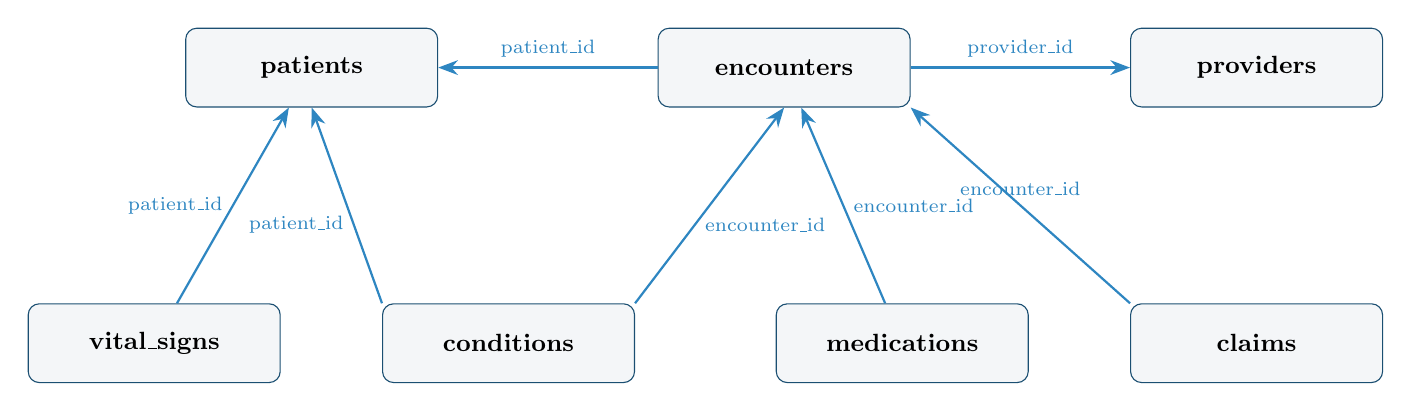
\begin{tikzpicture}[
    entity/.style={rectangle, rounded corners=4pt, draw=primary, fill=primary!5,
                   minimum width=3.2cm, minimum height=1cm, font=\small\bfseries,
                   align=center},
    rel/.style={-{Stealth[length=2.5mm]}, thick, color=secondary},
]

% Row 1: the two main parent tables + providers
\node[entity] (patients) at (0, 0) {patients};
\node[entity] (encounters) at (6, 0) {encounters};
\node[entity] (providers) at (12, 0) {providers};

% Row 2: children spread out horizontally with enough spacing
\node[entity] (vitals) at (-2, -3.5) {vital\_signs};
\node[entity] (conditions) at (2.5, -3.5) {conditions};
\node[entity] (medications) at (7.5, -3.5) {medications};
\node[entity] (claims) at (12, -3.5) {claims};

% encounters -> patients (FK: patient_id)
\draw[rel] (encounters) -- node[above, font=\scriptsize] {patient\_id} (patients);

% encounters -> providers (FK: provider_id)
\draw[rel] (encounters) -- node[above, font=\scriptsize] {provider\_id} (providers);

% vitals -> patients (FK: patient_id)
\draw[rel] (vitals) -- node[left, font=\scriptsize] {patient\_id} (patients);

% conditions -> patients (FK: patient_id)  --- clear diagonal, no overlap
\draw[rel] (conditions.north west) -- node[left, font=\scriptsize, pos=0.4] {patient\_id} (patients.south);

% conditions -> encounters (FK: encounter_id) --- clear diagonal, opposite side
\draw[rel] (conditions.north east) -- node[right, font=\scriptsize, pos=0.4] {encounter\_id} (encounters.south);

% medications -> encounters (FK: encounter_id)
\draw[rel] (medications) -- node[right, font=\scriptsize] {encounter\_id} (encounters);

% claims -> encounters (FK: encounter_id) --- clear line from right side
\draw[rel] (claims.north west) -- node[above, font=\scriptsize, pos=0.5] {encounter\_id} (encounters.south east);

\end{tikzpicture}%
}
\caption{OLTP Entity-Relationship Diagram --- arrows point from child to parent (FK direction)}
\label{fig:er-diagram}
\end{figure}

\begin{notebox}
    Reading the diagram: An arrow from \texttt{encounters} to \texttt{patients} means ``each encounter belongs to one patient'' (the \texttt{encounters} table has a \texttt{patient\_id} column that references \texttt{patients}). One patient can have many encounters --- this is a \textbf{one-to-many} relationship.
\end{notebox}

\section{Star Schema (Data Warehouse)}
\label{sec:star-schema}

The warehouse uses a \textbf{Star Schema}\index{Star Schema} --- the most common design for analytics databases.

\begin{conceptbox}{What Is a Star Schema?}
A Star Schema has two types of tables:
\begin{itemize}
    \item \textbf{Fact Tables}\index{Fact Table} (center of the star) --- contain \textit{measurements/metrics}: costs, counts, amounts. Each row is an ``event'' or ``transaction.''
    \item \textbf{Dimension Tables}\index{Dimension Table} (points of the star) --- contain \textit{descriptive attributes}: who, what, when, where. They give context to the facts.
\end{itemize}

It is called a ``star'' because when you draw the diagram, the fact table in the center connects to dimensions around it, forming a star shape.

\textbf{Why not just use 3NF for analytics?}
\begin{itemize}
    \item 3NF requires many JOINs, which slows down large analytical queries
    \item Star Schema needs fewer JOINs (usually just fact $\rightarrow$ dimension)
    \item Business users find star schemas intuitive: ``Give me \textit{total cost} (fact) by \textit{hospital} (dimension) for \textit{Q1 2024} (dimension)''
\end{itemize}

\textbf{A simple analogy:}
\begin{itemize}
    \item \textbf{Fact table} = A sales receipt (date, amount, product ID, customer ID)
    \item \textbf{Dimension tables} = Reference cards (product catalog, customer directory, calendar)
    \item To analyze sales, you join the receipt to the reference cards to get the full picture
\end{itemize}
\end{conceptbox}

\subsection{Fact Tables}

\begin{longtable}{>{\ttfamily\small}p{3cm} p{3cm} p{3cm} p{3.5cm}}
    \toprule
    \normalfont\textbf{Table} & \textbf{Grain} & \textbf{Measures} & \textbf{Dimension Keys} \\
    \midrule
    \endhead
    fact\_encounters & One row per hospital visit & total\_cost, length\_of\_stay, num\_conditions, readmission\_flag & patient\_key, provider\_key, date\_key, payer\_key \\
    \midrule
    fact\_claims & One row per insurance claim & amount\_billed, amount\_paid, amount\_denied, processing\_days & patient\_key, encounter\_key, payer\_key, date\_key \\
    \midrule
    fact\_vitals & One row per vital sign reading & heart\_rate, systolic\_bp, diastolic\_bp, temperature, spo2, anomaly\_flag & patient\_key, date\_key, time\_key \\
    \bottomrule
\end{longtable}

\begin{notebox}
    The \textbf{grain}\index{Grain} is the most important decision in fact table design. It answers: ``What does one row represent?'' Always define the grain \textit{before} choosing columns. A wrong grain leads to incorrect aggregations and misleading reports.

    \textbf{Example:} If the grain of \texttt{fact\_encounters} is ``one row per hospital visit,'' then a patient who visited 3 times has 3 rows. The \texttt{total\_cost} column holds the cost of \textit{that specific visit}, not the patient's total lifetime cost.
\end{notebox}

\subsection{Dimension Tables}

\begin{longtable}{>{\ttfamily\small}p{2.8cm} p{2cm} p{8cm}}
    \toprule
    \normalfont\textbf{Table} & \textbf{SCD Type} & \textbf{Key Columns} \\
    \midrule
    \endhead
    dim\_patient & Type 2 & patient\_key, patient\_id, name, birth\_date, gender, race, city, state, insurance\_type, valid\_from, valid\_to, is\_current \\
    \midrule
    dim\_provider & Type 2 & provider\_key, provider\_id, name, specialty, organization, valid\_from, valid\_to, is\_current \\
    \midrule
    dim\_date & Static & date\_key, full\_date, year, quarter, month, week, day\_of\_week, is\_weekend, is\_holiday, fiscal\_quarter \\
    \midrule
    dim\_time & Static & time\_key, hour, minute, am\_pm, shift (morning / afternoon / night) \\
    \midrule
    dim\_diagnosis & Type 1 & diagnosis\_key, icd10\_code, description, category, body\_system \\
    \midrule
    dim\_payer & Type 1 & payer\_key, payer\_name, payer\_type (private/public/self-pay), plan\_name \\
    \bottomrule
\end{longtable}

\begin{conceptbox}{What Are Slowly Changing Dimensions (SCD)?}
Real-world data changes over time. A patient might move to a new city or change their insurance. How do you handle that?

\textbf{SCD Type 1 --- Overwrite:}\index{SCD Type 1}
\begin{itemize}
    \item Simply update the old value with the new one
    \item You \textit{lose} the history: you cannot see what the old value was
    \item Good for: corrections, typo fixes, attributes you do not need to track historically
\end{itemize}

\textbf{Example:} A diagnosis description has a typo. You just fix it:
\begin{center}
\small
\begin{tabular}{ccc}
    \toprule
    \textbf{diagnosis\_key} & \textbf{description (before)} & \textbf{description (after)} \\
    \midrule
    501 & Diabtes Type 2 & Diabetes Type 2 \\
    \bottomrule
\end{tabular}
\end{center}

\textbf{SCD Type 2 --- Add a New Row:}\index{SCD Type 2}
\begin{itemize}
    \item Keep the old row (mark it as \texttt{is\_current = 0}, set \texttt{valid\_to = today})
    \item Insert a new row with updated values (\texttt{is\_current = 1}, \texttt{valid\_from = today})
    \item You \textit{preserve} the full history
    \item Good for: patient address, insurance plan, provider specialty --- anything you want to analyze historically
\end{itemize}

\textbf{Example:} Patient moves from Cairo to Alexandria on March 1:
\begin{center}
\small
\begin{tabular}{ccccc}
    \toprule
    \textbf{patient\_key} & \textbf{city} & \textbf{valid\_from} & \textbf{valid\_to} & \textbf{is\_current} \\
    \midrule
    101 & Cairo & 2020-01-01 & 2024-02-28 & 0 \\
    102 & Alexandria & 2024-03-01 & 9999-12-31 & 1 \\
    \bottomrule
\end{tabular}
\end{center}
Both rows have the same \texttt{patient\_id} (the business key), but different \texttt{patient\_key} (the surrogate key). An encounter on January 15 links to key 101 (Cairo), while an encounter on April 10 links to key 102 (Alexandria).

\textbf{Why does this matter?} If you analyze ``average cost by city,'' January encounters count toward Cairo and April encounters count toward Alexandria --- giving you \textit{historically accurate} results.
\end{conceptbox}

\subsection{Surrogate Keys vs.\ Business Keys}

\begin{conceptbox}{What Is a Surrogate Key?}
\begin{itemize}
    \item A \textbf{business key}\index{Business Key} is the natural identifier from the source system (e.g., \texttt{patient\_id} = UUID from the hospital)
    \item A \textbf{surrogate key}\index{Surrogate Key} is an artificial integer generated by the warehouse (e.g., \texttt{patient\_key} = 1, 2, 3, \ldots)
\end{itemize}

\textbf{Why use surrogate keys instead of business keys?}
\begin{enumerate}
    \item \textbf{Performance:} Integer JOINs are faster than UUID/string JOINs
    \item \textbf{SCD Type 2:} One \texttt{patient\_id} can have multiple \texttt{patient\_key} values (one per version)
    \item \textbf{Source independence:} If the source system changes its ID format, the warehouse is unaffected
\end{enumerate}
\end{conceptbox}

\subsection{Synapse Distribution Strategies}

Azure Synapse distributes data across 60 compute nodes. How you distribute matters for performance:

\begin{center}
\begin{tabular}{>{\bfseries}p{3cm} p{4.5cm} p{5cm}}
    \toprule
    \textbf{Strategy} & \textbf{How It Works} & \textbf{We Use It For} \\
    \midrule
    HASH & Rows with the same key value go to the same node & Fact tables (HASH on patient\_key) --- keeps related data together \\
    REPLICATE & Full copy on every node & Dimension tables (they are small) --- avoids shuffling during JOINs \\
    \bottomrule
\end{tabular}
\end{center}

\begin{tipbox}
    \textbf{Rule of thumb:} HASH-distribute large fact tables on the column you JOIN on most often (usually the main dimension key). REPLICATE small dimension tables so every node has a local copy and never needs to request data from other nodes.
\end{tipbox}

\begin{exercisebox}
\textbf{Practice:}
\begin{enumerate}
    \item A patient named Sara had insurance with ``National Insurance Co.'' until June 2024, then switched to ``HealthPlus.'' Draw the SCD Type 2 rows that would exist in \texttt{dim\_patient} for Sara.
    \item The \texttt{fact\_encounters} table has the grain ``one row per hospital visit.'' If you wanted a table tracking ``one row per medication prescribed,'' what would you name it and what measures might it have?
    \item Why is \texttt{dim\_date} marked as ``Static'' (not SCD Type 1 or 2)? Think about whether dates ever change.
\end{enumerate}
\end{exercisebox}

\begin{summarybox}
\textbf{Key Takeaways:}
\begin{itemize}
    \item OLTP uses 3NF (normalized) for efficient writes; OLAP uses Star Schema (denormalized) for efficient reads
    \item Star Schema consists of fact tables (measurements) surrounded by dimension tables (context)
    \item The grain defines what one row in a fact table represents --- always define it first
    \item SCD Type 1 overwrites old values; SCD Type 2 preserves history with versioned rows
    \item Surrogate keys (integers) are used instead of business keys for performance and SCD support
    \item In Synapse: HASH-distribute large fact tables, REPLICATE small dimension tables
\end{itemize}
\end{summarybox}


% ============================================================================
% CHAPTER 5: DATA SOURCES AND GENERATION
% ============================================================================
\chapter{Data Sources --- Where the Data Comes From}
\label{ch:datasources}

\begin{objectivebox}
By the end of this chapter, you will be able to:
\begin{itemize}
    \item Explain why we use synthetic data instead of real patient data
    \item Describe each of the four data sources and what they produce
    \item Interpret medical coding standards (ICD-10, SNOMED CT, RxNorm)
    \item Understand normal vital sign ranges and what anomalies look like
    \item Explain what a REST API is and how the Provider API works
\end{itemize}
\end{objectivebox}

Since this is a capstone project, we cannot use real patient data (privacy laws like HIPAA\index{HIPAA} forbid it). Instead, we generate \textbf{realistic synthetic data} from four sources.

\section{Source 1: Synthea (Patient Records)}

\textbf{Synthea}\index{Synthea} is an open-source tool by MITRE that generates realistic (but completely fictional) patient medical records.

\begin{itemize}
    \item \textbf{Output:} CSV files for patients, encounters, conditions, medications, and more
    \item \textbf{Volume:} 100,000 patients, which generates $\sim$500K encounters and 300K conditions
    \item \textbf{Medical accuracy:} Uses real clinical pathways --- if a patient has diabetes, Synthea generates realistic medication sequences and complications
    \item \textbf{Standards:} Uses ICD-10 codes (diagnoses), SNOMED CT (clinical terms), RxNorm (medications)
\end{itemize}

\begin{conceptbox}{Medical Coding Standards --- Quick Reference}
Hospitals worldwide use standardized codes so that different systems can understand each other:
\begin{itemize}
    \item \textbf{ICD-10:}\index{ICD-10} International Classification of Diseases. Example: \texttt{E11.9} = Type 2 diabetes without complications. Used for billing and diagnosis tracking.
    \item \textbf{SNOMED CT:}\index{SNOMED CT} A comprehensive clinical terminology. More detailed than ICD-10. Used in electronic health records.
    \item \textbf{RxNorm:}\index{RxNorm} Standard names for medications. Example: ``Metformin 500mg oral tablet'' instead of brand names like ``Glucophage.''
\end{itemize}
These standards ensure data is consistent and interoperable across hospital systems.
\end{conceptbox}

\section{Source 2: Custom Claims Generator (Python + Faker)}

The \texttt{generate\_claims.py} script creates fake insurance claims using the \textbf{Faker}\index{Faker} library.

\textbf{What it generates:}
\begin{itemize}
    \item 200,000 insurance claims
    \item Each claim has: payer name, amount billed, amount paid, claim status
    \item Statuses: \texttt{submitted}, \texttt{approved}, \texttt{denied}, \texttt{appealed}, \texttt{paid}
    \item Realistic denial rate: 15--20\% of claims are denied (matching real-world patterns)
    \item Multiple payer types: private insurance, public (government), self-pay
\end{itemize}

\begin{tipbox}
    \textbf{Why realistic distributions matter:} If 100\% of claims were ``approved,'' our dashboards would show no useful insights. By modeling real-world patterns (15--20\% denial rate, varying costs by encounter type), the data tells a realistic story that exercises all our analytical queries.
\end{tipbox}

\section{Source 3: Vital Signs Simulator (IoT Stream)}

The \texttt{simulate\_vitals.py} script simulates IoT\index{IoT} medical devices sending patient vital signs in real-time.

\textbf{Normal vital sign ranges:}
\begin{center}
\small
\begin{tabular}{p{3cm} c p{3cm} p{4.5cm}}
    \toprule
    \textbf{Vital Sign} & \textbf{Normal Range} & \textbf{Unit} & \textbf{What It Measures} \\
    \midrule
    Heart Rate & 60--100 & bpm & How fast the heart beats \\
    Systolic BP & 90--120 & mmHg & Pressure when heart contracts \\
    Diastolic BP & 60--80 & mmHg & Pressure when heart relaxes \\
    Temperature & 36.5--37.5 & \textdegree C & Core body temperature \\
    SpO2 & 95--100 & \% & Oxygen level in the blood \\
    \bottomrule
\end{tabular}
\end{center}

\textbf{Injected anomalies (for testing anomaly detection):}
\begin{itemize}
    \item \textbf{Tachycardia spikes} --- Heart rate jumps above 120 bpm (fast heartbeat)
    \item \textbf{Hypotension episodes} --- Systolic blood pressure drops below 90 mmHg (dangerously low)
    \item \textbf{Fever patterns} --- Temperature exceeds 38.5\textdegree C
\end{itemize}

\begin{notebox}
    The simulator deliberately injects about 5--10\% anomalous readings so that the anomaly detection pipeline in Databricks has something to find. Without these injected anomalies, we would have nothing to test our alerting system against.
\end{notebox}

\section{Source 4: Provider API (Flask REST API)}

The \texttt{provider\_api.py} runs a simple web API that serves doctor/provider information.

\textbf{Endpoints:}
\begin{center}
\begin{tabular}{l l p{6cm}}
    \toprule
    \textbf{Method} & \textbf{Endpoint} & \textbf{Returns} \\
    \midrule
    GET & \texttt{/providers} & List of all providers (JSON array) \\
    GET & \texttt{/providers/\{id\}} & Details for a specific provider (JSON object) \\
    GET & \texttt{/providers?specialty=cardiology} & Providers filtered by specialty \\
    \bottomrule
\end{tabular}
\end{center}

\begin{conceptbox}{What Is a REST API?}
A \textbf{REST API}\index{REST API} (Representational State Transfer Application Programming Interface) is a way for programs to communicate over HTTP (the same protocol your web browser uses).

\textbf{How it works:}
\begin{enumerate}[label=\textcolor{primary}{\arabic*.}]
    \item Your program sends an HTTP \textbf{request} to a URL (e.g., \texttt{GET /providers})
    \item The server processes the request
    \item The server sends back a \textbf{response} containing structured data (usually JSON)
\end{enumerate}

\textbf{Example:} When you visit \texttt{http://localhost:5000/providers/123}, instead of getting an HTML web page, you get structured JSON data:
\begin{lstlisting}[style=pythonstyle]
{
    "provider_id": "123",
    "name": "Dr. Ahmed Mohamed",
    "specialty": "Cardiology",
    "organization": "Cairo General Hospital"
}
\end{lstlisting}
This JSON data can be easily read by other programs, dashboards, or data pipelines.
\end{conceptbox}

\begin{summarybox}
\textbf{Key Takeaways:}
\begin{itemize}
    \item We use synthetic data because real patient data is protected by privacy laws (HIPAA)
    \item Synthea generates 100K realistic patients with proper medical coding (ICD-10, RxNorm)
    \item The claims generator creates 200K claims with realistic approval/denial patterns
    \item The vitals simulator produces real-time data with intentional anomalies for testing
    \item The Provider API serves data via REST endpoints that other systems can consume
\end{itemize}
\end{summarybox}


% ============================================================================
% CHAPTER 6: DOCKER
% ============================================================================
\chapter{Docker --- Running the Local Environment}
\label{ch:docker}

\begin{objectivebox}
By the end of this chapter, you will be able to:
\begin{itemize}
    \item Explain what Docker is and why it solves the ``works on my machine'' problem
    \item Define key Docker vocabulary: image, container, Dockerfile, volume
    \item Read and understand a \texttt{docker-compose.yml} file
    \item Read and understand a \texttt{Dockerfile}
    \item Start, stop, and debug the project's Docker services
\end{itemize}
\end{objectivebox}

\section{What Is Docker and Why Do We Use It?}

\begin{conceptbox}{Docker in Simple Terms}
Imagine you wrote a Python script that works perfectly on your laptop. You give it to your teammate, and it crashes because they have a different Python version, missing libraries, or a different operating system.

\textbf{Docker}\index{Docker} solves this by packaging your application \textit{with everything it needs} (OS, libraries, configuration) into a \textbf{container}. A container is like a lightweight virtual computer that runs identically on any machine.

Key vocabulary:
\begin{itemize}
    \item \textbf{Image}\index{Docker!Image} = The blueprint/recipe (like a class in OOP)
    \item \textbf{Container}\index{Docker!Container} = A running instance of an image (like an object)
    \item \textbf{Dockerfile}\index{Dockerfile} = Instructions to build an image (like a recipe)
    \item \textbf{docker-compose.yml} = Defines and runs multiple containers together
    \item \textbf{Volume}\index{Docker!Volume} = Persistent storage that survives container restarts
\end{itemize}

\textbf{Analogy:} Think of a Docker image as a recipe for a cake. You can bake (run) that recipe to get a cake (container). You can bake the same recipe on any oven (machine) and get the same cake. If you want to keep the cake fresh between baking sessions, you put it in the fridge (volume).
\end{conceptbox}

\section{Our Docker Setup}

We have two files in the \texttt{docker/} folder:

\subsection{docker-compose.yml --- Defining Our Services}

This file defines \textbf{two services} that work together:

\begin{lstlisting}[style=yamlstyle, caption={docker/docker-compose.yml}]
version: "3.8"

services:
  sqlserver:
    image: mcr.microsoft.com/mssql/server:2022-latest
    container_name: healthcare_sqlserver
    environment:
      ACCEPT_EULA: "Y"
      MSSQL_SA_PASSWORD: ${MSSQL_SA_PASSWORD:-YourStrong!Passw0rd}
      MSSQL_PID: Developer
    ports:
      - "1433:1433"
    volumes:
      - sqlserver_data:/var/opt/mssql
    healthcheck:
      test: /opt/mssql-tools18/bin/sqlcmd -S localhost
            -U sa -P "$${MSSQL_SA_PASSWORD}"
            -C -Q "SELECT 1" -b -o /dev/null
      interval: 10s
      timeout: 5s
      retries: 10
      start_period: 30s

  data-generator:
    build:
      context: ..
      dockerfile: docker/Dockerfile.generator
    container_name: healthcare_generator
    depends_on:
      sqlserver:
        condition: service_healthy
    env_file:
      - ../.env
    ports:
      - "5000:5000"

volumes:
  sqlserver_data:
\end{lstlisting}

\textbf{Line-by-line explanation:}

\begin{enumerate}[label=\textcolor{primary}{\textbf{\arabic*.}}]
    \item \texttt{version: "3.8"} --- The Docker Compose file format version

    \item \textbf{Service: sqlserver}
    \begin{itemize}
        \item \texttt{image: mcr.microsoft.com/mssql/server:2022-latest} --- Downloads the official SQL Server 2022 image from Microsoft
        \item \texttt{ACCEPT\_EULA: "Y"} --- Accepts the license agreement (required)
        \item \texttt{MSSQL\_SA\_PASSWORD} --- The \texttt{sa} (system admin) password. Uses value from \texttt{.env} file, defaults to \texttt{YourStrong!Passw0rd}
        \item \texttt{MSSQL\_PID: Developer} --- Uses the free Developer Edition
        \item \texttt{ports: "1433:1433"} --- Maps port 1433 in the container to port 1433 on your machine (1433 is the standard SQL Server port)
        \item \texttt{volumes: sqlserver\_data} --- Stores database files in a persistent volume so data survives container restarts
        \item \texttt{healthcheck} --- Runs a SQL query (\texttt{SELECT 1}) every 10 seconds to verify the database is ready. Other services wait for this before starting.
    \end{itemize}

    \item \textbf{Service: data-generator}
    \begin{itemize}
        \item \texttt{build: context/dockerfile} --- Builds from \texttt{Dockerfile.generator} (explained next)
        \item \texttt{depends\_on: service\_healthy} --- Waits until SQL Server's healthcheck passes before starting
        \item \texttt{env\_file: ../.env} --- Loads environment variables from the \texttt{.env} file
        \item \texttt{ports: "5000:5000"} --- Exposes the Flask API on port 5000
    \end{itemize}
\end{enumerate}

\subsection{Dockerfile.generator --- Building the Python Image}

\begin{lstlisting}[style=dockerstyle, caption={docker/Dockerfile.generator}]
FROM python:3.11-slim

RUN apt-get update && \
    apt-get install -y --no-install-recommends \
        curl \
        gnupg2 \
        unixodbc-dev && \
    curl -fsSL https://packages.microsoft.com/keys/microsoft.asc \
        | gpg --dearmor -o /usr/share/keyrings/microsoft-prod.gpg && \
    curl -fsSL https://packages.microsoft.com/config/debian/12/prod.list \
        | tee /etc/apt/sources.list.d/mssql-release.list && \
    apt-get update && \
    ACCEPT_EULA=Y apt-get install -y msodbcsql18 && \
    apt-get clean && \
    rm -rf /var/lib/apt/lists/*

WORKDIR /app

COPY requirements.txt .
RUN pip install --no-cache-dir -r requirements.txt

COPY src/ ./src/
COPY config/ ./config/

EXPOSE 5000

CMD ["python", "src/generators/provider_api.py"]
\end{lstlisting}

\textbf{What each instruction does:}

\begin{enumerate}[label=\textcolor{primary}{\textbf{\arabic*.}}]
    \item \texttt{FROM python:3.11-slim} --- Start from a minimal Python 3.11 image (``slim'' means fewer unnecessary packages, smaller image)
    \item \texttt{RUN apt-get \ldots} --- Install system dependencies:
    \begin{itemize}
        \item \texttt{curl, gnupg2} --- tools to download and verify Microsoft's package signing key
        \item \texttt{unixodbc-dev} --- ODBC driver manager (needed to connect to SQL Server)
        \item \texttt{msodbcsql18} --- Microsoft's ODBC Driver 18 for SQL Server
    \end{itemize}
    \item \texttt{WORKDIR /app} --- Set the working directory inside the container
    \item \texttt{COPY requirements.txt \& pip install} --- Install Python dependencies \textit{before} copying source code (this is a Docker best practice --- if your code changes but dependencies do not, Docker reuses the cached layer)
    \item \texttt{COPY src/ \& config/} --- Copy your application code into the container
    \item \texttt{EXPOSE 5000} --- Document that this container listens on port 5000
    \item \texttt{CMD} --- The default command when the container starts
\end{enumerate}

\begin{tipbox}
    \textbf{Docker Layer Caching:} Each instruction in a Dockerfile creates a ``layer.'' Docker caches layers and only rebuilds from the first changed instruction downward. By copying \texttt{requirements.txt} and installing dependencies \textit{before} copying source code, we avoid reinstalling all packages every time we change a line of Python code. This makes builds much faster during development.
\end{tipbox}

\section{How to Use Docker in This Project}

\begin{lstlisting}[style=bashstyle, caption={Docker commands for local development}]
# Start both services (SQL Server + data generator)
docker-compose -f docker/docker-compose.yml up -d

# Check if services are running
docker ps

# View logs from the data generator
docker logs healthcare_generator

# View logs from SQL Server
docker logs healthcare_sqlserver

# Stop all services
docker-compose -f docker/docker-compose.yml down

# Stop and DELETE all data (fresh start)
docker-compose -f docker/docker-compose.yml down -v
\end{lstlisting}

\begin{warningbox}
    The \texttt{-v} flag in the last command deletes the persistent volume, which means \textbf{all database data is lost}. Only use it when you want a completely fresh start.
\end{warningbox}

\begin{exercisebox}
\textbf{Practice:}
\begin{enumerate}
    \item Run \texttt{docker ps} on your machine. What containers are currently running (if any)?
    \item In the \texttt{docker-compose.yml}, what would happen if you removed the \texttt{healthcheck} section? \textit{(Hint: think about the \texttt{depends\_on} condition)}
    \item The Dockerfile installs the ODBC driver for SQL Server. Why is this needed inside the Python container?
\end{enumerate}
\end{exercisebox}

\begin{summarybox}
\textbf{Key Takeaways:}
\begin{itemize}
    \item Docker packages applications with all dependencies into portable containers
    \item Images are blueprints; containers are running instances; volumes persist data
    \item Our setup runs SQL Server 2022 and a Python data generator as two linked services
    \item The healthcheck ensures SQL Server is ready before the generator starts
    \item Docker layer caching speeds up builds by reusing unchanged layers
\end{itemize}
\end{summarybox}


% ============================================================================
% CHAPTER 7: ENVIRONMENT CONFIGURATION
% ============================================================================
\chapter{Configuration --- Environment Variables and Dependencies}
\label{ch:config}

\begin{objectivebox}
By the end of this chapter, you will be able to:
\begin{itemize}
    \item Explain why configuration should be separated from code
    \item Set up the \texttt{.env} file from the provided template
    \item Understand each environment variable group and what it connects to
    \item Install Python dependencies from \texttt{requirements.txt}
    \item Configure code quality tools (flake8, pytest) via \texttt{setup.cfg}
\end{itemize}
\end{objectivebox}

\section{Why Environment Variables?}

Hardcoding passwords and connection strings directly in your code is dangerous:
\begin{itemize}
    \item If you push code to GitHub, everyone can see your passwords
    \item Different environments (development, staging, production) need different values
    \item Changing a password means changing code, rebuilding, and redeploying
\end{itemize}

\textbf{Environment variables}\index{Environment Variables} solve this by storing configuration \textit{outside} your code, in a \texttt{.env} file that is \textbf{never committed to Git}.

\begin{conceptbox}{The Twelve-Factor App Principle}
This approach follows a well-known software engineering principle from the \textbf{Twelve-Factor App} methodology: ``Store config in the environment.'' The idea is that your code should be identical in development and production --- only the \textit{configuration} (connection strings, passwords, feature flags) should differ.
\end{conceptbox}

\section{The .env.example File}

This is the \textit{template} that shows what variables you need to set. It is safe to commit because it does not contain real secrets.

\begin{lstlisting}[style=bashstyle, caption={.env.example --- the template (safe to share)}]
# SQL Server (Local Development)
MSSQL_HOST=localhost
MSSQL_PORT=1433
MSSQL_DB=healthcare_oltp
MSSQL_USER=sa
MSSQL_SA_PASSWORD=YourStrong!Passw0rd
MSSQL_DRIVER=ODBC Driver 18 for SQL Server

# Azure Data Lake Storage Gen2
ADLS_ACCOUNT_NAME=your_storage_account
ADLS_ACCOUNT_KEY=your_account_key
ADLS_CONTAINER_BRONZE=bronze
ADLS_CONTAINER_SILVER=silver
ADLS_CONTAINER_GOLD=gold

# Azure Event Hubs
EVENT_HUB_CONNECTION_STRING=your_connection_string
EVENT_HUB_NAME=vitals-stream

# Azure Synapse Analytics
SYNAPSE_SERVER=your_workspace.sql.azuresynapse.net
SYNAPSE_DATABASE=healthcare_dw
SYNAPSE_USER=your_username
SYNAPSE_PASSWORD=your_password

# Databricks
DATABRICKS_HOST=https://your-workspace.azuredatabricks.net
DATABRICKS_TOKEN=your_token

# Flask API
FLASK_HOST=0.0.0.0
FLASK_PORT=5000
FLASK_DEBUG=False
\end{lstlisting}

\textbf{Variable groups explained:}

\begin{enumerate}[label=\textcolor{primary}{\textbf{\arabic*.}}]
    \item \textbf{SQL Server} --- Connection to the local Docker SQL Server (OLTP source)
    \item \textbf{Azure Data Lake} --- Cloud storage credentials. Bronze/Silver/Gold are container names matching our Medallion layers
    \item \textbf{Event Hubs} --- Connection for the real-time vitals streaming pipeline
    \item \textbf{Synapse} --- Connection to the cloud data warehouse (Gold layer target)
    \item \textbf{Databricks} --- Connection to the Spark processing cluster
    \item \textbf{Flask} --- Configuration for the Provider API service
\end{enumerate}

\begin{importantbox}
    \textbf{To set up your environment:}
    \begin{enumerate}
        \item Copy the template: \texttt{cp .env.example .env}
        \item Edit \texttt{.env} with your actual values
        \item \textbf{Never} commit \texttt{.env} to Git (it is in \texttt{.gitignore})
    \end{enumerate}
\end{importantbox}

\section{Python Dependencies (requirements.txt)}

This file lists every Python package the project needs, with minimum version numbers:

\begin{lstlisting}[style=bashstyle, caption={requirements.txt --- organized by purpose}]
# Data Processing
pandas>=2.1.0          # DataFrames for tabular data
numpy>=1.25.0          # Numerical operations
pyarrow>=14.0.0        # Read/write Parquet files

# Data Generation
faker>=20.0.0          # Generate fake data (names, dates, etc.)

# Database (SQL Server)
sqlalchemy>=2.0.0      # Python SQL toolkit and ORM
pyodbc>=5.0.0          # ODBC database connector
pymssql>=2.2.11        # Alternative SQL Server connector

# API
flask>=3.0.0           # Lightweight web framework
requests>=2.31.0       # HTTP client library

# Spark (local development)
pyspark>=3.5.0         # Apache Spark Python API
delta-spark>=3.0.0     # Delta Lake for Spark

# Visualization
matplotlib>=3.8.0      # Static charts and plots
seaborn>=0.13.0        # Statistical visualization
plotly>=5.18.0         # Interactive charts

# EDA & Profiling
ydata-profiling>=4.6.0 # Auto-generate data reports

# Streaming
azure-eventhub>=5.11.0 # Azure Event Hubs client

# Azure SDK
azure-storage-file-datalake>=12.14.0  # Data Lake client
azure-identity>=1.15.0                # Azure authentication

# Testing
pytest>=7.4.0          # Test framework
flake8>=6.1.0          # Code style checker

# Streamlit (optional)
streamlit>=1.29.0      # Web dashboard framework
\end{lstlisting}

\textbf{To install all dependencies:}
\begin{lstlisting}[style=bashstyle]
pip install -r requirements.txt
\end{lstlisting}

\begin{tipbox}
    The \texttt{>=} syntax means ``this version or newer.'' For example, \texttt{pandas>=2.1.0} installs pandas 2.1.0 or any later version. This ensures you get bug fixes while maintaining compatibility. For production projects, you might use \texttt{==} (exact version) for fully reproducible builds.
\end{tipbox}

\section{Code Quality Configuration (setup.cfg)}

\begin{lstlisting}[style=bashstyle, caption={setup.cfg --- linting and testing rules}]
[flake8]
max-line-length = 120
exclude = .git,__pycache__,venv,.venv,data
ignore = E203,W503

[tool:pytest]
testpaths = tests
python_files = test_*.py
python_functions = test_*
\end{lstlisting}

\begin{itemize}
    \item \textbf{flake8}\index{flake8} --- A Python code style checker (``linter''):
    \begin{itemize}
        \item \texttt{max-line-length = 120} --- Lines must not exceed 120 characters
        \item \texttt{exclude} --- Skip checking these folders
        \item \texttt{ignore = E203, W503} --- Ignore two specific style rules that conflict with the Black formatter
    \end{itemize}
    \item \textbf{pytest}\index{pytest} --- The testing framework:
    \begin{itemize}
        \item \texttt{testpaths = tests} --- Look for tests in the \texttt{tests/} folder
        \item \texttt{python\_files = test\_*.py} --- Test files must start with \texttt{test\_}
        \item \texttt{python\_functions = test\_*} --- Test functions must start with \texttt{test\_}
    \end{itemize}
\end{itemize}

\begin{summarybox}
\textbf{Key Takeaways:}
\begin{itemize}
    \item Never hardcode secrets --- use environment variables stored in a \texttt{.env} file
    \item The \texttt{.env.example} is a safe template; the actual \texttt{.env} is Git-ignored
    \item \texttt{requirements.txt} lists all Python packages with minimum versions
    \item \texttt{setup.cfg} configures code linting (flake8) and test discovery (pytest)
\end{itemize}
\end{summarybox}


% ============================================================================
% CHAPTER 8: CI/CD PIPELINE
% ============================================================================
\chapter{CI/CD Pipeline --- Automated Quality Checks}
\label{ch:cicd}

\begin{objectivebox}
By the end of this chapter, you will be able to:
\begin{itemize}
    \item Define CI (Continuous Integration) and CD (Continuous Deployment)
    \item Read and understand a GitHub Actions workflow YAML file
    \item Explain each job in our CI pipeline and how they depend on each other
    \item Interpret CI pipeline results on GitHub (passing/failing checks)
\end{itemize}
\end{objectivebox}

\section{What Is CI/CD?}

\begin{conceptbox}{CI/CD in Simple Terms}
\textbf{CI} (Continuous Integration)\index{Continuous Integration}\index{CI|see{Continuous Integration}} means: every time someone pushes code, automated checks run immediately to catch problems early.

\textbf{CD} (Continuous Deployment/Delivery)\index{Continuous Deployment} means: if all checks pass, the code is automatically deployed.

Think of it as a quality control inspector on a factory assembly line --- every product (code change) is checked before it moves to the next station.

We use \textbf{GitHub Actions}\index{GitHub Actions} --- a free CI/CD service built into GitHub.

\textbf{Without CI:} A developer pushes broken code $\rightarrow$ nobody notices $\rightarrow$ other developers pull broken code $\rightarrow$ everyone wastes time debugging.

\textbf{With CI:} A developer pushes broken code $\rightarrow$ automated tests fail within minutes $\rightarrow$ the developer is notified immediately $\rightarrow$ they fix it before anyone else is affected.
\end{conceptbox}

\section{Our Pipeline Configuration}

The pipeline is defined in \texttt{.github/workflows/ci.yml}:

\begin{lstlisting}[style=yamlstyle, caption={.github/workflows/ci.yml --- our CI pipeline}]
name: CI Pipeline

on:
  push:
    branches: [main, develop]
  pull_request:
    branches: [main]

jobs:
  lint:
    name: Python Linting
    runs-on: ubuntu-latest
    steps:
      - uses: actions/checkout@v4
      - uses: actions/setup-python@v5
        with:
          python-version: "3.11"
      - run: pip install flake8
      - run: flake8 src/ tests/ --max-line-length=120
                     --exclude=__pycache__

  test:
    name: Unit Tests
    runs-on: ubuntu-latest
    needs: lint
    steps:
      - uses: actions/checkout@v4
      - uses: actions/setup-python@v5
        with:
          python-version: "3.11"
      - run: pip install -r requirements.txt
      - run: pytest tests/ -v --tb=short

  sql-lint:
    name: SQL Validation
    runs-on: ubuntu-latest
    steps:
      - uses: actions/checkout@v4
      - run: pip install sqlfluff
      - run: sqlfluff lint sql/ --dialect tsql || true
\end{lstlisting}

\section{Pipeline Flow Explained}

\begin{figure}[H]
\centering
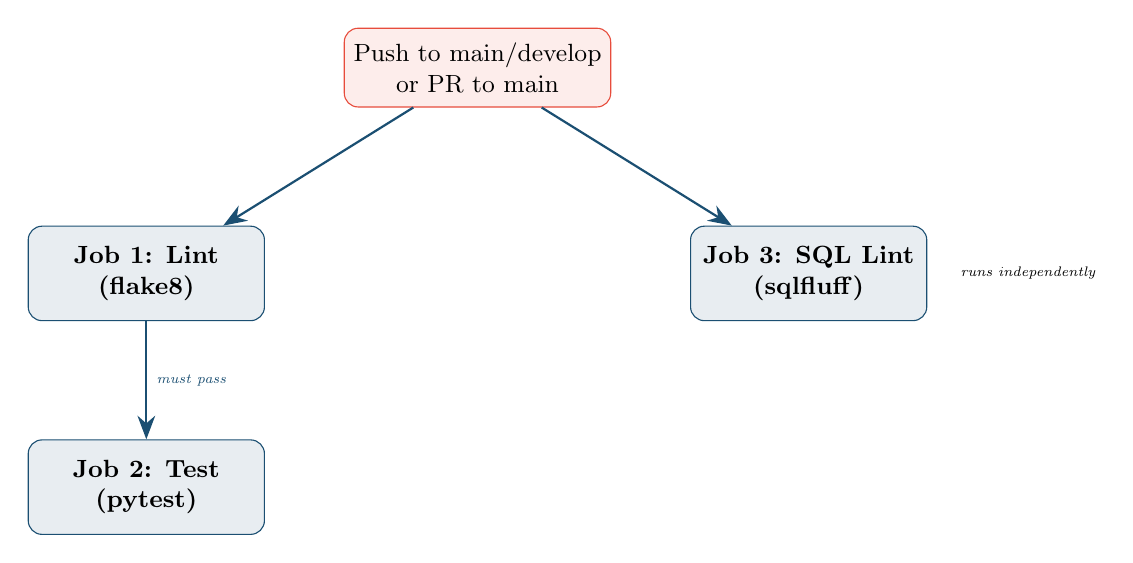
\begin{tikzpicture}[
    node distance=1.5cm and 2cm,
    job/.style={rectangle, rounded corners=5pt, draw=primary, fill=primary!10,
                minimum width=3cm, minimum height=1.2cm, font=\small\bfseries,
                align=center},
    trigger/.style={rectangle, rounded corners=5pt, draw=accent, fill=accent!10,
                    minimum width=3cm, minimum height=1cm, font=\small,
                    align=center},
    arrow/.style={-{Stealth[length=3mm]}, thick, color=primary}
]

\node[trigger] (push) {Push to main/develop\\or PR to main};

\node[job, below left=1.5cm and 1cm of push] (lint) {Job 1: Lint\\(flake8)};
\node[job, below right=1.5cm and 1cm of push] (sqllint) {Job 3: SQL Lint\\(sqlfluff)};
\node[job, below=1.5cm of lint] (test) {Job 2: Test\\(pytest)};

\draw[arrow] (push) -- (lint);
\draw[arrow] (push) -- (sqllint);
\draw[arrow] (lint) -- node[right, font=\tiny\itshape] {must pass} (test);

\node[font=\tiny\itshape, right=0.3cm of sqllint] {runs independently};

\end{tikzpicture}
\caption{CI Pipeline execution flow}
\label{fig:ci-pipeline}
\end{figure}

\subsection{Job 1: Python Linting (flake8)}

\begin{itemize}
    \item \textbf{Triggers:} Runs on every push and PR
    \item \textbf{What it does:} Checks Python code style --- line length, unused imports, syntax errors
    \item \textbf{If it fails:} Job 2 (tests) will not run
\end{itemize}

\subsection{Job 2: Unit Tests (pytest)}

\begin{itemize}
    \item \textbf{Triggers:} Only runs \textit{after} linting passes (\texttt{needs: lint})
    \item \textbf{What it does:} Runs all tests in \texttt{tests/} folder
    \item \textbf{Flags:} \texttt{-v} (verbose output), \texttt{--tb=short} (short error tracebacks)
\end{itemize}

\subsection{Job 3: SQL Validation (sqlfluff)}

\begin{itemize}
    \item \textbf{Triggers:} Runs in parallel with Job 1 (independent)
    \item \textbf{What it does:} Checks SQL files for style and syntax issues using T-SQL dialect
    \item \textbf{Note:} The \texttt{|| true} means it will not fail the pipeline even if SQL issues are found (soft enforcement for now)
\end{itemize}

\begin{notebox}
    \textbf{Reading the YAML file:}
    \begin{itemize}
        \item \texttt{on:} defines \textit{when} the pipeline runs (push to main/develop, or PR to main)
        \item \texttt{jobs:} defines \textit{what} runs. Each job runs on a fresh virtual machine (\texttt{ubuntu-latest})
        \item \texttt{steps:} are the sequential commands within a job
        \item \texttt{needs: lint} means ``wait for the lint job to finish successfully first''
        \item \texttt{uses:} refers to pre-built GitHub Actions (like ``checkout code'' or ``install Python'')
    \end{itemize}
\end{notebox}

\begin{summarybox}
\textbf{Key Takeaways:}
\begin{itemize}
    \item CI automatically runs checks (linting, tests) on every code push to catch bugs early
    \item Our pipeline has 3 jobs: Python linting, unit tests, and SQL validation
    \item Jobs can depend on each other (\texttt{needs:}) or run in parallel
    \item GitHub Actions workflows are defined in YAML files under \texttt{.github/workflows/}
\end{itemize}
\end{summarybox}


% ============================================================================
% CHAPTER 9: TESTING
% ============================================================================
\chapter{Testing --- Verifying the Project Works}
\label{ch:testing}

\begin{objectivebox}
By the end of this chapter, you will be able to:
\begin{itemize}
    \item Explain why automated testing is important in software projects
    \item Read and understand pytest test functions
    \item Run tests locally and interpret the output
    \item Understand what each test in our suite verifies
\end{itemize}
\end{objectivebox}

\section{Why Test?}

Testing prevents the ``it works on my machine'' problem. Automated tests:
\begin{itemize}
    \item Catch bugs \textit{before} they reach production
    \item Give you confidence to change code without breaking things
    \item Serve as documentation --- tests show how code is \textit{supposed} to work
    \item Run automatically in CI (Chapter~\ref{ch:cicd}) on every push
\end{itemize}

\begin{conceptbox}{Types of Tests}
\begin{itemize}
    \item \textbf{Unit tests}\index{Unit Test} --- Test a single function or method in isolation. Fast, focused. \textit{Example: ``Does the date parser handle invalid dates correctly?''}
    \item \textbf{Integration tests}\index{Integration Test} --- Test that multiple components work together. \textit{Example: ``Can the generator write data to SQL Server successfully?''}
    \item \textbf{End-to-end tests} --- Test the entire system from input to output. \textit{Example: ``Does data flow from Bronze to Gold correctly?''}
\end{itemize}
Our current test suite focuses on \textbf{scaffold validation} --- verifying the project structure is correct. As the project grows, we will add unit and integration tests for each component.
\end{conceptbox}

\section{Our Test Suite}

Currently, the project has \textbf{scaffold validation tests} that verify the project structure is set up correctly. These run in CI on every push.

\begin{lstlisting}[style=pythonstyle, caption={tests/test\_project\_structure.py}]
import os

ROOT_DIR = os.path.dirname(
    os.path.dirname(os.path.abspath(__file__))
)

def test_required_directories_exist():
    """Verify all expected project directories exist."""
    expected_dirs = [
        "src",
        "src/generators",
        "src/synthea",
        "notebooks",
        "sql",
        "sql/ddl",
        "sql/queries",
        "pipelines",
        "dashboards",
        "docs",
        "tests",
        "docker",
        "config",
    ]
    for d in expected_dirs:
        path = os.path.join(ROOT_DIR, d)
        assert os.path.isdir(path), f"Missing directory: {d}"


def test_required_files_exist():
    """Verify all critical files are present."""
    expected_files = [
        "README.md",
        "requirements.txt",
        ".env.example",
        ".gitignore",
        "setup.cfg",
        "docker/docker-compose.yml",
        "docker/Dockerfile.generator",
        ".github/workflows/ci.yml",
    ]
    for f in expected_files:
        path = os.path.join(ROOT_DIR, f)
        assert os.path.isfile(path), f"Missing file: {f}"


def test_env_example_has_required_keys():
    """Verify .env.example has all required variables."""
    env_path = os.path.join(ROOT_DIR, ".env.example")
    with open(env_path, "r") as f:
        content = f.read()

    required_keys = [
        "MSSQL_HOST",
        "MSSQL_PORT",
        "MSSQL_DB",
        "ADLS_ACCOUNT_NAME",
        "EVENT_HUB_CONNECTION_STRING",
        "SYNAPSE_SERVER",
        "FLASK_PORT",
    ]
    for key in required_keys:
        assert key in content, f"Missing env key: {key}"


def test_requirements_has_core_packages():
    """Verify requirements.txt has essential packages."""
    req_path = os.path.join(ROOT_DIR, "requirements.txt")
    with open(req_path, "r") as f:
        content = f.read()

    core_packages = [
        "pandas",
        "pyspark",
        "faker",
        "sqlalchemy",
        "pyodbc",
        "flask",
        "pytest",
    ]
    for pkg in core_packages:
        assert pkg in content, f"Missing package: {pkg}"
\end{lstlisting}

\subsection{Understanding Each Test}

\begin{enumerate}[label=\textcolor{primary}{\textbf{Test \arabic*:}}]
    \item \textbf{test\_required\_directories\_exist()} --- Loops through 13 expected directories and checks each one exists using \texttt{os.path.isdir()}. If any is missing, the test fails with a clear message like ``Missing directory: sql/ddl''.

    \textbf{Line-by-line breakdown:}
    \begin{itemize}
        \item \texttt{ROOT\_DIR} is calculated by going up two levels from the test file to reach the project root
        \item \texttt{os.path.join(ROOT\_DIR, d)} builds the full path to each directory
        \item \texttt{assert os.path.isdir(path)} checks the directory exists --- if not, the test fails with the message after the comma
    \end{itemize}

    \item \textbf{test\_required\_files\_exist()} --- Same pattern but for 8 critical files (README, requirements, Docker files, CI config). Uses \texttt{os.path.isfile()} instead of \texttt{isdir()}.

    \item \textbf{test\_env\_example\_has\_required\_keys()} --- Reads the entire \texttt{.env.example} file as a string, then checks that 7 key variable names appear in the text. This ensures the template is complete.

    \item \textbf{test\_requirements\_has\_core\_packages()} --- Reads \texttt{requirements.txt} and checks that 7 essential package names are present. This ensures no one accidentally deletes a dependency.
\end{enumerate}

\section{Running Tests Locally}

\begin{lstlisting}[style=bashstyle, caption={How to run tests}]
# Run all tests with verbose output
pytest tests/ -v

# Run a specific test file
pytest tests/test_project_structure.py -v

# Run a specific test function
pytest tests/test_project_structure.py::test_required_files_exist -v

# Run with short error output
pytest tests/ -v --tb=short
\end{lstlisting}

\textbf{Expected output when all tests pass:}
\begin{lstlisting}[style=bashstyle]
tests/test_project_structure.py::test_required_directories_exist PASSED
tests/test_project_structure.py::test_required_files_exist PASSED
tests/test_project_structure.py::test_env_example_has_required_keys PASSED
tests/test_project_structure.py::test_requirements_has_core_packages PASSED

========= 4 passed in 0.05s =========
\end{lstlisting}

\begin{tipbox}
    If any test fails, read the error message carefully. It will tell you exactly what is missing (e.g., ``Missing directory: sql/ddl''). Create the missing item and re-run. The \texttt{--tb=short} flag gives you a concise error traceback without pages of detail.
\end{tipbox}

\begin{summarybox}
\textbf{Key Takeaways:}
\begin{itemize}
    \item Tests catch bugs early, provide confidence for refactoring, and serve as documentation
    \item Our 4 scaffold tests verify: directories exist, files exist, \texttt{.env.example} is complete, and \texttt{requirements.txt} has all packages
    \item Use \texttt{pytest tests/ -v} to run all tests with verbose output
    \item Tests run automatically in CI on every push via GitHub Actions
\end{itemize}
\end{summarybox}


% ============================================================================
% CHAPTER 10: GIT AND VERSION CONTROL
% ============================================================================
\chapter{Git and Version Control}
\label{ch:git}

\begin{objectivebox}
By the end of this chapter, you will be able to:
\begin{itemize}
    \item Explain core Git concepts: repository, commit, branch, merge
    \item Understand what \texttt{.gitignore} and \texttt{.gitattributes} do
    \item Follow the feature-branch workflow used in this project
    \item Write proper commit messages using conventional prefixes
\end{itemize}
\end{objectivebox}

\section{Git Basics for This Project}

If you are new to Git, here is the minimum you need to know:

\begin{conceptbox}{Git in 60 Seconds}
\textbf{Git}\index{Git} tracks every change to every file in your project. Think of it as an ``infinite undo'' button with named checkpoints (called \textit{commits}).

Key concepts:
\begin{itemize}
    \item \textbf{Repository (repo)} = Your project folder, tracked by Git
    \item \textbf{Commit} = A snapshot of all files at a point in time (like a save point in a video game)
    \item \textbf{Branch} = A parallel version of the code (like a copy you can experiment with)
    \item \textbf{main} = The primary branch with stable, reviewed code
    \item \textbf{develop} = The integration branch where features are merged before going to main
    \item \textbf{Pull Request (PR)} = A request to merge your branch into main/develop, with code review
\end{itemize}

\textbf{Visual analogy:} Imagine a tree. The \texttt{main} branch is the trunk. When you create a feature branch, you grow a new limb. When the feature is done and reviewed, you merge it back into the trunk.
\end{conceptbox}

\section{The .gitignore File}

This file tells Git which files to \textbf{never track}. Our \texttt{.gitignore} excludes:

\begin{lstlisting}[style=bashstyle, caption={Key sections of .gitignore}]
# Python caches (auto-generated, not needed)
__pycache__/
*.py[cod]

# Environment variables (contains secrets!)
.env
*.env.local

# Data files (too large for Git)
data/raw/*.csv
data/raw/*.json
data/raw/*.parquet
data/cleaned/*.parquet
data/gold/*.parquet

# Power BI files (binary, large)
*.pbix
*.pbit

# IDE settings (personal preference)
.vscode/
.idea/

# Virtual environment (can be recreated)
venv/
.venv/
\end{lstlisting}

\begin{importantbox}
    The most critical line is \texttt{.env} --- this prevents your passwords and API keys from being pushed to GitHub where anyone can see them. \textbf{Always verify \texttt{.env} is in your \texttt{.gitignore} before pushing.}
\end{importantbox}

\section{The .gitattributes File}

This file ensures consistent behavior across Windows, Mac, and Linux:

\begin{itemize}
    \item \textbf{Text files} (Python, SQL, YAML, Markdown) --- use LF (Unix) line endings
    \item \textbf{Windows scripts} (.bat, .ps1) --- use CRLF (Windows) line endings
    \item \textbf{Binary files} (.parquet, .pbix, .png) --- treated as binary (no line ending conversion)
\end{itemize}

\begin{tipbox}
    Windows uses \texttt{CRLF} (Carriage Return + Line Feed, two characters) for line endings, while Mac/Linux use just \texttt{LF} (one character). Without \texttt{.gitattributes}, Git might show every line as changed when switching between operating systems. This file prevents that confusion.
\end{tipbox}

\section{Common Git Workflow}

\begin{lstlisting}[style=bashstyle, caption={Daily Git workflow}]
# 1. Create a feature branch
git checkout -b feature/add-claims-generator

# 2. Make your changes...
# 3. Check what you changed
git status
git diff

# 4. Stage specific files
git add src/generators/generate_claims.py
git add tests/test_claims_generator.py

# 5. Commit with a descriptive message
git commit -m "feat: add claims data generator with Faker"

# 6. Push to remote
git push -u origin feature/add-claims-generator

# 7. Create a Pull Request on GitHub
# 8. After review and approval, merge to develop
\end{lstlisting}

\begin{notebox}
    \textbf{Commit message prefixes:}
    \begin{itemize}
        \item \texttt{feat:} --- New feature
        \item \texttt{fix:} --- Bug fix
        \item \texttt{docs:} --- Documentation changes
        \item \texttt{test:} --- Adding or updating tests
        \item \texttt{refactor:} --- Code restructuring (no new features)
        \item \texttt{chore:} --- Build process, dependencies, config changes
    \end{itemize}
    These prefixes follow the \textbf{Conventional Commits} standard and make it easy to scan the Git history and understand what each change did.
\end{notebox}

\begin{summarybox}
\textbf{Key Takeaways:}
\begin{itemize}
    \item Git tracks all changes with commits (snapshots) and branches (parallel versions)
    \item \texttt{.gitignore} prevents secrets and large files from being committed
    \item \texttt{.gitattributes} ensures consistent line endings across operating systems
    \item Follow the feature-branch workflow: create branch $\rightarrow$ code $\rightarrow$ commit $\rightarrow$ push $\rightarrow$ PR $\rightarrow$ review $\rightarrow$ merge
    \item Use conventional commit prefixes (feat, fix, docs, test, refactor, chore)
\end{itemize}
\end{summarybox}


% ============================================================================
% CHAPTER 11: ANALYTICAL QUERIES
% ============================================================================
\chapter{Analytical SQL Queries}
\label{ch:queries}

\begin{objectivebox}
By the end of this chapter, you will be able to:
\begin{itemize}
    \item List the 10 analytical queries included in this project
    \item Explain window functions (LAG, RANK, NTILE) and how they differ from GROUP BY
    \item Read and understand a CTE-based query step by step
    \item Trace through the 30-day readmission rate query and explain each part
    \item Understand GROUPING SETS for multi-level aggregation
\end{itemize}
\end{objectivebox}

The project includes \textbf{10+ analytical queries} designed to answer real business questions. Each query demonstrates different SQL techniques. Here are all of them:

\begin{longtable}{c >{\bfseries}p{3.5cm} p{4cm} p{4.5cm}}
    \toprule
    \textbf{\#} & \textbf{Query} & \textbf{SQL Techniques} & \textbf{Business Question} \\
    \midrule
    \endhead
    1 & 30-Day Readmission Rate & LAG(), DATEDIFF, CTE, CASE & Which conditions cause the most readmissions? \\
    \midrule
    2 & Patient Cost Distribution & NTILE(), PERCENTILE\_CONT, window aggregation & How are costs distributed across patient segments? \\
    \midrule
    3 & Provider Performance & RANK(), DENSE\_RANK(), AVG OVER & Which providers have the best outcomes? \\
    \midrule
    4 & Condition Co-occurrence & Self-JOIN, CROSS APPLY, PIVOT & Which conditions frequently appear together? \\
    \midrule
    5 & Monthly Encounter Trends & DATE\_TRUNC, LAG(), running total & Are encounter volumes increasing or decreasing? \\
    \midrule
    6 & Claim Denial Analysis & GROUPING SETS, HAVING, ratios & What is the denial rate by payer? \\
    \midrule
    7 & Length of Stay Analysis & DATEDIFF, CASE, MEDIAN, outliers & Average length of stay by condition? \\
    \midrule
    8 & Patient Cohort Retention & Date arithmetic, cohort assignment, PIVOT & How do patient cohorts retain over time? \\
    \midrule
    9 & Top Medications by Cost & SUM, RANK(), cumulative \% (Pareto) & Which medications drive the most cost? \\
    \midrule
    10 & Vital Signs Anomaly Summary & WHERE anomaly\_flag=1, time patterns & When do most anomalies occur? \\
    \bottomrule
\end{longtable}

\section{Key SQL Concepts Explained}

Before diving into the queries, let us understand the key SQL concepts they use.

\begin{conceptbox}{Window Functions --- The Most Powerful SQL Feature}
\textbf{Window functions}\index{Window Function} perform calculations across a set of rows \textit{related to} the current row, without collapsing them into a single output row.

\textbf{How they differ from GROUP BY:}
\begin{itemize}
    \item \textbf{GROUP BY} collapses rows: 1000 rows $\rightarrow$ 10 groups $\rightarrow$ 10 output rows
    \item \textbf{Window functions} keep all rows: 1000 rows $\rightarrow$ 1000 output rows, each with an extra computed column
\end{itemize}

\textbf{Syntax pattern:}
\begin{lstlisting}[style=sqlstyle]
function_name() OVER (
    PARTITION BY column  -- divide rows into groups
    ORDER BY column      -- order within each group
)
\end{lstlisting}

\textbf{Common window functions:}
\begin{itemize}
    \item \texttt{LAG(col, n)} --- Get the value from \texttt{n} rows \textit{before} the current row
    \item \texttt{LEAD(col, n)} --- Get the value from \texttt{n} rows \textit{after} the current row
    \item \texttt{RANK()} --- Assign a rank (1, 2, 2, 4 --- ties get same rank, next rank is skipped)
    \item \texttt{DENSE\_RANK()} --- Like RANK but no gaps (1, 2, 2, 3)
    \item \texttt{NTILE(n)} --- Divide rows into \texttt{n} equal groups (quartiles, deciles, etc.)
    \item \texttt{SUM() OVER()} --- Running total or group total without collapsing
\end{itemize}

\textbf{Simple example:}
\begin{lstlisting}[style=sqlstyle]
-- For each patient, show their visit date AND their previous visit date
SELECT
    patient_id,
    visit_date,
    LAG(visit_date, 1) OVER (
        PARTITION BY patient_id   -- group by patient
        ORDER BY visit_date       -- sort by date within each patient
    ) AS previous_visit_date
FROM encounters;
\end{lstlisting}
Result: each row now has both the current visit date and the previous one, making it easy to calculate gaps between visits.
\end{conceptbox}

\begin{conceptbox}{Common Table Expressions (CTEs)}
A \textbf{CTE}\index{CTE} (Common Table Expression) is a named temporary result set that exists only for the duration of a single query. It is defined with \texttt{WITH ... AS (...)}.

\textbf{Why use CTEs?}
\begin{itemize}
    \item Break complex queries into readable, named steps
    \item Each CTE can reference previous CTEs
    \item Much easier to debug than deeply nested subqueries
\end{itemize}

\textbf{Simple example:}
\begin{lstlisting}[style=sqlstyle]
-- Without CTE (hard to read):
SELECT * FROM (
    SELECT *, ROW_NUMBER() OVER(PARTITION BY dept ORDER BY salary DESC) rn
    FROM employees
) sub WHERE rn = 1;

-- With CTE (easy to read):
WITH ranked_employees AS (
    SELECT *,
        ROW_NUMBER() OVER(PARTITION BY dept ORDER BY salary DESC) AS rn
    FROM employees
)
SELECT * FROM ranked_employees WHERE rn = 1;
\end{lstlisting}
Both queries do the same thing (find the highest-paid employee in each department), but the CTE version clearly labels what each step does.
\end{conceptbox}

\section{Deep Dive: 30-Day Readmission Rate}

This query identifies patients who returned to the hospital within 30 days of discharge --- a key quality metric in healthcare:

\begin{lstlisting}[style=sqlstyle, caption={Readmission rate query pattern}]
WITH encounter_pairs AS (
    SELECT
        fe.patient_key,
        fe.date_key AS current_visit,
        LAG(fe.date_key) OVER (
            PARTITION BY fe.patient_key
            ORDER BY dd.full_date
        ) AS previous_visit,
        dd.full_date AS visit_date,
        fe.length_of_stay_days
    FROM fact_encounters fe
    JOIN dim_date dd ON fe.date_key = dd.date_key
),
readmissions AS (
    SELECT *,
        DATEDIFF(DAY, previous_visit_date, visit_date)
            AS days_since_last_visit,
        CASE
            WHEN DATEDIFF(DAY, previous_visit_date, visit_date) <= 30
            THEN 1
            ELSE 0
        END AS is_readmission
    FROM encounter_pairs
    WHERE previous_visit IS NOT NULL
)
SELECT
    COUNT(*) AS total_encounters,
    SUM(is_readmission) AS readmissions,
    CAST(SUM(is_readmission) AS FLOAT) / COUNT(*)
        AS readmission_rate
FROM readmissions;
\end{lstlisting}

\textbf{Step-by-step walkthrough:}

\begin{enumerate}[label=\textcolor{primary}{\textbf{Step \arabic*:}}]
    \item \textbf{CTE 1 --- encounter\_pairs:} For each patient's encounters (sorted by date), use \texttt{LAG()} to look back at the \textit{previous} visit date. This pairs each visit with the one before it.

    \textit{What LAG does here:} If patient \#42 visited on Jan 5, Feb 10, and Mar 20, the result is:
    \begin{center}
    \small
    \begin{tabular}{ccc}
        \toprule
        \textbf{visit\_date} & \textbf{previous\_visit} & \textbf{gap} \\
        \midrule
        Jan 5 & NULL & --- \\
        Feb 10 & Jan 5 & 36 days \\
        Mar 20 & Feb 10 & 38 days \\
        \bottomrule
    \end{tabular}
    \end{center}

    \item \textbf{CTE 2 --- readmissions:} Calculate the number of days between consecutive visits using \texttt{DATEDIFF}. Then use \texttt{CASE} to flag any gap $\leq$ 30 days as a readmission (\texttt{is\_readmission = 1}). Rows with no previous visit (\texttt{NULL}) are filtered out.

    \item \textbf{Final SELECT:} Count total encounters, sum the readmission flags, and divide to get the rate. \texttt{CAST(... AS FLOAT)} ensures decimal division (otherwise SQL does integer division: \texttt{3/10 = 0} instead of \texttt{0.3}).
\end{enumerate}

\begin{tipbox}
    \textbf{Why does this matter clinically?} A high 30-day readmission rate may indicate:
    \begin{itemize}
        \item Patients being discharged too early
        \item Inadequate follow-up care after discharge
        \item Specific conditions that need better treatment protocols
    \end{itemize}
    Hospitals are sometimes penalized financially for high readmission rates, making this metric critically important.
\end{tipbox}

\begin{summarybox}
\textbf{Key Takeaways:}
\begin{itemize}
    \item The project includes 10+ SQL queries covering readmissions, costs, provider performance, anomalies, and more
    \item Window functions (LAG, RANK, NTILE) compute values across related rows without collapsing them
    \item CTEs break complex queries into named, readable steps
    \item The readmission query uses LAG to pair consecutive visits, DATEDIFF to measure gaps, and CASE to flag readmissions
\end{itemize}
\end{summarybox}


% ============================================================================
% CHAPTER 12: AZURE CLOUD SERVICES
% ============================================================================
\chapter{Azure Cloud Services --- What Each Service Does}
\label{ch:azure}

\begin{objectivebox}
By the end of this chapter, you will be able to:
\begin{itemize}
    \item Name the 5 Azure services used in this project and explain each one's role
    \item Describe how data flows between Azure services
    \item Explain what a Synapse dedicated SQL pool is and why it uses 60 distributions
    \item Understand what columnstore indexes are and why they speed up analytics
\end{itemize}
\end{objectivebox}

This chapter explains each Azure service we use and how it fits into the pipeline. Do not worry about Azure pricing or setup details --- focus on understanding \textit{what each service does} and \textit{why we chose it}.

\section{Azure Data Lake Storage Gen2}

\begin{itemize}
    \item \textbf{What it is:} A cloud storage service optimized for big data analytics
    \item \textbf{Think of it as:} A huge, organized file system in the cloud (like a network drive with unlimited space)
    \item \textbf{Our use:} Store raw (Bronze), cleaned (Silver), and final (Gold) data files
    \item \textbf{Key feature:} Hierarchical namespace --- you can organize files into folders, just like on your computer
    \item \textbf{Containers:} \texttt{bronze}, \texttt{silver}, \texttt{gold} (one per Medallion layer)
\end{itemize}

\section{Azure Data Factory (ADF)}

\begin{itemize}
    \item \textbf{What it is:} A cloud-based data integration (ETL\index{ETL}) service
    \item \textbf{Think of it as:} A delivery truck scheduler --- it moves data between systems on a schedule
    \item \textbf{Our use:} Copy data from Data Lake (Bronze) into Databricks for processing
    \item \textbf{Key concepts:}
    \begin{itemize}
        \item \textbf{Pipeline} = A workflow with multiple steps
        \item \textbf{Activity} = A single step (e.g., Copy Data, Run Notebook)
        \item \textbf{Trigger} = When to run (schedule, event-based)
        \item \textbf{Linked Service} = Connection to an external system (Data Lake, Databricks, etc.)
    \end{itemize}
\end{itemize}

\section{Azure Databricks}

\begin{itemize}
    \item \textbf{What it is:} A managed Apache Spark\index{Apache Spark} platform
    \item \textbf{Think of it as:} A powerful computer cluster that processes massive datasets using PySpark
    \item \textbf{Our use:}
    \begin{itemize}
        \item \textbf{Silver processing:} Cleaning, deduplication, schema enforcement
        \item \textbf{Gold transformation:} Building the Star Schema, calculating KPIs
        \item \textbf{Streaming:} Spark Structured Streaming for real-time vitals
    \end{itemize}
    \item \textbf{Key feature:} Notebooks --- interactive code environments similar to Jupyter, but running on a Spark cluster with distributed processing power
\end{itemize}

\begin{conceptbox}{What Is Apache Spark?}
\textbf{Apache Spark}\index{Apache Spark} is a distributed data processing engine. Instead of processing data on one computer, Spark splits the work across many computers (a ``cluster'') working in parallel.

\textbf{Why do we need it?}
\begin{itemize}
    \item Processing 500K encounters on one computer: maybe 10 minutes
    \item Processing 500K encounters on a 10-node Spark cluster: maybe 1 minute
    \item For real-world hospitals with billions of records, Spark is essential
\end{itemize}

\textbf{PySpark} is the Python API for Spark --- you write Python code, and Spark distributes it across the cluster automatically.
\end{conceptbox}

\section{Azure Event Hubs}

\begin{itemize}
    \item \textbf{What it is:} A big data streaming platform and event ingestion service
    \item \textbf{Think of it as:} A high-speed mail slot that can receive millions of messages per second
    \item \textbf{Our use:} Receives real-time vital sign readings from the IoT simulator
    \item \textbf{Key concept:} Producers (our Python simulator) \textit{send} events; consumers (Spark Streaming) \textit{read} events
\end{itemize}

\section{Azure Synapse Analytics}

\begin{itemize}
    \item \textbf{What it is:} An enterprise analytics service (cloud data warehouse)
    \item \textbf{Think of it as:} A super-powered SQL Server designed for analytics queries on huge datasets
    \item \textbf{Our use:} Hosts the Gold layer Star Schema --- Power BI connects here for dashboards
    \item \textbf{Key features:}
    \begin{itemize}
        \item \textbf{Dedicated SQL Pool} --- Reserved compute nodes always available
        \item \textbf{60 distributions} --- Data is automatically spread across 60 nodes for parallel processing
        \item \textbf{Columnstore indexes}\index{Columnstore Index} --- Compresses data and speeds up analytical queries by 10--100x
    \end{itemize}
\end{itemize}

\begin{conceptbox}{What Are Columnstore Indexes?}
Traditional databases store data \textbf{row by row} (like reading a book line by line). Columnstore indexes store data \textbf{column by column}.

\textbf{Why does this matter for analytics?}

When you run \texttt{SELECT AVG(total\_cost) FROM fact\_encounters}, the database only needs the \texttt{total\_cost} column. With row storage, it must read \textit{every column} of every row to find the one it needs. With columnstore, it reads \textit{only} the \texttt{total\_cost} column --- skipping everything else.

\textbf{Benefits:}
\begin{itemize}
    \item \textbf{10--100x faster} for analytical queries (reads less data)
    \item \textbf{10x better compression} (similar values in a column compress well)
    \item \textbf{Perfect for} SUM, AVG, COUNT, GROUP BY queries on large tables
\end{itemize}
\end{conceptbox}

\section{How Services Connect}

\begin{figure}[H]
\centering
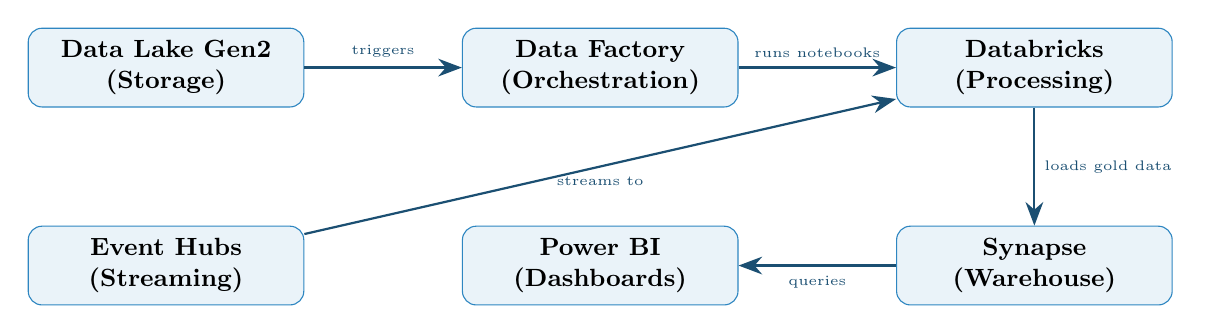
\begin{tikzpicture}[
    node distance=1.5cm,
    service/.style={rectangle, rounded corners=5pt, draw=secondary, fill=secondary!10,
                    minimum width=3.5cm, minimum height=1cm, font=\small\bfseries,
                    align=center},
    arrow/.style={-{Stealth[length=3mm]}, thick, color=primary},
]

\node[service] (adls) {Data Lake Gen2\\(Storage)};
\node[service, right=2cm of adls] (adf) {Data Factory\\(Orchestration)};
\node[service, right=2cm of adf] (dbricks) {Databricks\\(Processing)};
\node[service, below=1.5cm of dbricks] (synapse) {Synapse\\(Warehouse)};
\node[service, below=1.5cm of adls] (ehubs) {Event Hubs\\(Streaming)};
\node[service, left=2cm of synapse] (pbi) {Power BI\\(Dashboards)};

\draw[arrow] (adls) -- node[above, font=\tiny] {triggers} (adf);
\draw[arrow] (adf) -- node[above, font=\tiny] {runs notebooks} (dbricks);
\draw[arrow] (dbricks) -- node[right, font=\tiny] {loads gold data} (synapse);
\draw[arrow] (synapse) -- node[below, font=\tiny] {queries} (pbi);
\draw[arrow] (ehubs) -- node[below, font=\tiny] {streams to} (dbricks);

\end{tikzpicture}
\caption{Azure service interconnections}
\label{fig:azure-services}
\end{figure}

\begin{summarybox}
\textbf{Key Takeaways:}
\begin{itemize}
    \item \textbf{Data Lake Gen2} = cloud file storage (Bronze/Silver/Gold containers)
    \item \textbf{Data Factory} = orchestration/scheduling (moves data between services)
    \item \textbf{Databricks} = Spark-based processing (cleaning, transformation, streaming)
    \item \textbf{Event Hubs} = real-time event ingestion (receives IoT vital signs)
    \item \textbf{Synapse} = cloud data warehouse (hosts Gold layer, serves Power BI)
    \item Columnstore indexes speed up analytical queries by reading only needed columns
\end{itemize}
\end{summarybox}


% ============================================================================
% CHAPTER 13: GETTING STARTED
% ============================================================================
\chapter{Getting Started --- Step-by-Step Setup}
\label{ch:setup}

\begin{objectivebox}
By the end of this chapter, you will be able to:
\begin{itemize}
    \item Install all prerequisites (Python, Git, Docker, Java, Azure CLI)
    \item Clone the repository and set up a virtual environment
    \item Configure environment variables and install dependencies
    \item Start Docker services and verify everything works
    \item Run the data generators
\end{itemize}
\end{objectivebox}

Follow these steps \textit{in order} to set up the project on your machine.

\section{Prerequisites}

Before you begin, install these tools:

\begin{enumerate}[label=\textcolor{primary}{\textbf{\arabic*.}}]
    \item \textbf{Python 3.11+} --- \url{https://python.org/downloads}
    \begin{itemize}
        \item During installation on Windows, check ``Add Python to PATH''
    \end{itemize}

    \item \textbf{Git} --- \url{https://git-scm.com/downloads}

    \item \textbf{Docker Desktop} --- \url{https://docker.com/products/docker-desktop}
    \begin{itemize}
        \item On Windows, this requires WSL2 (Windows Subsystem for Linux)
        \item Docker Desktop will guide you through the WSL2 setup
    \end{itemize}

    \item \textbf{Java 11+} (for Synthea) --- \url{https://adoptium.net}

    \item \textbf{Azure CLI} (for cloud deployment) --- \url{https://aka.ms/installazurecliwindows}

    \item \textbf{A code editor} --- VS Code is recommended (\url{https://code.visualstudio.com})
\end{enumerate}

\begin{tipbox}
    You can verify each installation by running these commands in your terminal:
    \begin{lstlisting}[style=bashstyle]
python --version    # Should show 3.11+
git --version       # Should show 2.x+
docker --version    # Should show 20.x+
java --version      # Should show 11+
az --version        # Should show Azure CLI version
    \end{lstlisting}
\end{tipbox}

\section{Step 1: Clone the Repository}

\begin{lstlisting}[style=bashstyle]
git clone https://github.com/ma7moudalysalem/healthcare-data-warehouse.git
cd healthcare-data-warehouse
\end{lstlisting}

\begin{notebox}
    If you do not have access to the repository, ask the team lead (Mahmoud Salem) to add your GitHub username as a collaborator.
\end{notebox}

\section{Step 2: Create a Virtual Environment}

A \textbf{virtual environment}\index{Virtual Environment} isolates this project's Python packages from your system Python. This prevents conflicts between projects that need different package versions.

\begin{lstlisting}[style=bashstyle]
# Create the virtual environment
python -m venv venv

# Activate it
# On Windows (Command Prompt):
venv\Scripts\activate
# On Windows (PowerShell):
.\venv\Scripts\Activate.ps1
# On Mac/Linux:
source venv/bin/activate

# You should see (venv) at the start of your terminal prompt
\end{lstlisting}

\section{Step 3: Install Python Dependencies}

\begin{lstlisting}[style=bashstyle]
pip install -r requirements.txt
\end{lstlisting}

This installs all 20+ packages listed in \texttt{requirements.txt}. It may take a few minutes.

\section{Step 4: Configure Environment Variables}

\begin{lstlisting}[style=bashstyle]
# Copy the template
cp .env.example .env

# Edit with your favorite editor
code .env    # VS Code
notepad .env # Windows Notepad
\end{lstlisting}

For local development, you only need to change the \texttt{MSSQL\_SA\_PASSWORD}. Azure variables are needed later for cloud deployment.

\section{Step 5: Start Docker Services}

\begin{lstlisting}[style=bashstyle]
# Start SQL Server and the data generator
docker-compose -f docker/docker-compose.yml up -d

# Verify both containers are running
docker ps

# Wait for SQL Server to be healthy (may take 30-60 seconds)
docker logs healthcare_sqlserver
\end{lstlisting}

\section{Step 6: Run Tests}

\begin{lstlisting}[style=bashstyle]
# Verify everything is set up correctly
pytest tests/ -v
\end{lstlisting}

You should see all 4 tests passing:
\begin{lstlisting}[style=bashstyle]
tests/test_project_structure.py::test_required_directories_exist PASSED
tests/test_project_structure.py::test_required_files_exist PASSED
tests/test_project_structure.py::test_env_example_has_required_keys PASSED
tests/test_project_structure.py::test_requirements_has_core_packages PASSED

========= 4 passed in 0.05s =========
\end{lstlisting}

\begin{tipbox}
    If any test fails, read the error message carefully. It will tell you exactly what is missing (e.g., ``Missing directory: sql/ddl''). Create the missing item and re-run.
\end{tipbox}

\section{Step 7: Run the Data Generators}

\begin{lstlisting}[style=bashstyle]
# Generate synthetic claims data
python src/generators/generate_claims.py

# Start the vital signs simulator
python src/generators/simulate_vitals.py

# Start the provider API
python src/generators/provider_api.py
# API will be available at http://localhost:5000
\end{lstlisting}

\section{Quick Reference Card}

\begin{center}
\begin{tabular}{>{\ttfamily\small}p{7cm} p{6cm}}
    \toprule
    \normalfont\textbf{Command} & \textbf{What It Does} \\
    \midrule
    pytest tests/ -v & Run all tests \\
    flake8 src/ tests/ & Check code style \\
    docker-compose -f docker/\newline docker-compose.yml up -d & Start local services \\
    docker-compose -f docker/\newline docker-compose.yml down & Stop local services \\
    pip install -r requirements.txt & Install dependencies \\
    python src/generators/\newline provider\_api.py & Start the Flask API \\
    git status & Check modified files \\
    git add . \&\& git commit -m "msg" & Save changes \\
    \bottomrule
\end{tabular}
\end{center}

\begin{summarybox}
\textbf{Key Takeaways:}
\begin{itemize}
    \item Setup follows 7 sequential steps: clone $\rightarrow$ venv $\rightarrow$ install $\rightarrow$ configure $\rightarrow$ Docker $\rightarrow$ test $\rightarrow$ generate
    \item Always use a virtual environment to isolate Python packages
    \item Docker services must be healthy before running data generators that depend on SQL Server
    \item All 4 tests should pass before proceeding to development
\end{itemize}
\end{summarybox}


% ============================================================================
% CHAPTER 14: PROJECT MILESTONES
% ============================================================================
\chapter{Project Milestones and Timeline}
\label{ch:milestones}

\begin{objectivebox}
By the end of this chapter, you will be able to:
\begin{itemize}
    \item Describe the 5 project milestones and their deliverables
    \item Understand how each milestone builds on the previous one
    \item Identify which milestone you should be working on based on the timeline
\end{itemize}
\end{objectivebox}

The project is divided into \textbf{5 milestones} over \textbf{10 weeks}. Each milestone builds on the previous one.

\begin{figure}[H]
\centering
\resizebox{\textwidth}{!}{%
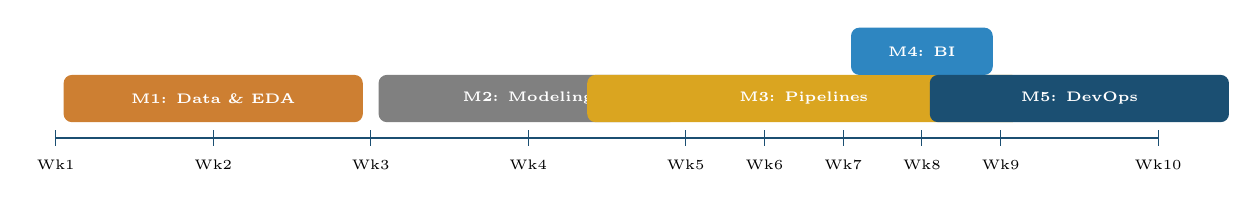
\begin{tikzpicture}[
    node distance=0.3cm,
    milestone/.style={rectangle, rounded corners=3pt, minimum width=2.2cm,
                      minimum height=0.6cm, font=\tiny\bfseries, text=white,
                      align=center},
]
% Timeline bar
\draw[thick, primary] (0,0) -- (14,0);
\foreach \x/\w in {0/Wk1, 2/Wk2, 4/Wk3, 6/Wk4, 8/Wk5, 9/Wk6, 10/Wk7, 11/Wk8, 12/Wk9, 14/Wk10} {
    \draw[primary] (\x, -0.1) -- (\x, 0.1);
    \node[below, font=\tiny] at (\x, -0.15) {\w};
}
% Milestone blocks
\node[milestone, fill=bronzecolor, minimum width=3.8cm] at (2, 0.5) {M1: Data \& EDA};
\node[milestone, fill=silvercolor, minimum width=3.8cm] at (6, 0.5) {M2: Modeling};
\node[milestone, fill=goldcolor, minimum width=5.5cm] at (9.5, 0.5) {M3: Pipelines};
\node[milestone, fill=secondary, minimum width=1.8cm] at (11, 1.1) {M4: BI};
\node[milestone, fill=primary, minimum width=3.8cm] at (13, 0.5) {M5: DevOps};
\end{tikzpicture}%
}
\caption{Project timeline --- 5 milestones over 10 weeks}
\label{fig:timeline}
\end{figure}

\section{Milestone 1: Data Collection \& EDA (Weeks 1--2)}

\textbf{Goal:} Generate all data sources and understand the data through exploratory analysis.

\textbf{Deliverables:}
\begin{enumerate}[label=\ding{51}]
    \item Configure Synthea to generate 100K patient records
    \item Build the claims generator (\texttt{generate\_claims.py})
    \item Build the vitals simulator (\texttt{simulate\_vitals.py})
    \item Build the provider API (\texttt{provider\_api.py})
    \item Create an EDA notebook with 15+ visualizations
    \item Design the ER diagram for the OLTP schema
    \item Write SQL DDL scripts for source tables
\end{enumerate}

\section{Milestone 2: Data Modeling \& Warehouse (Weeks 3--4)}

\textbf{Goal:} Design and build the Star Schema in Azure Synapse.

\textbf{Deliverables:}
\begin{enumerate}[label=\ding{51}]
    \item Design the Star Schema (fact and dimension tables)
    \item Write Synapse DDL scripts with proper distribution strategies
    \item Implement SCD Type 2 for patient and provider dimensions
    \item Write 10+ analytical SQL queries
    \item Create the data dictionary (every column documented)
\end{enumerate}

\section{Milestone 3: Pipelines --- Batch + Stream (Weeks 5--7)}

\textbf{Goal:} Build the complete data pipeline from source to warehouse.

\textbf{Deliverables:}
\begin{enumerate}[label=\ding{51}]
    \item Configure Azure Data Factory pipelines (Copy Activities)
    \item Build Databricks PySpark notebooks for Silver layer processing
    \item Build Databricks notebooks for Gold layer transformation
    \item Implement Spark Structured Streaming for vital signs
    \item Build anomaly detection logic
    \item Verify Delta Lake tables with time travel queries
\end{enumerate}

\section{Milestone 4: BI Dashboards (Week 8)}

\textbf{Goal:} Create interactive dashboards for business users.

\textbf{Deliverables:}
\begin{enumerate}[label=\ding{51}]
    \item Power BI Dashboard Page 1: Hospital Utilization
    \item Power BI Dashboard Page 2: Readmission Analysis
    \item Power BI Dashboard Page 3: Cost Analysis
    \item DAX measures for KPIs (readmission rate, average cost, etc.)
    \item Optional: Streamlit real-time monitoring dashboard
\end{enumerate}

\section{Milestone 5: DevOps \& Presentation (Weeks 9--10)}

\textbf{Goal:} Production-readiness, documentation, and final presentation.

\textbf{Deliverables:}
\begin{enumerate}[label=\ding{51}]
    \item CI/CD pipeline with GitHub Actions
    \item Docker containerization
    \item Azure Monitor and alerting setup
    \item Final project report
    \item Presentation slides
\end{enumerate}

\begin{summarybox}
\textbf{Key Takeaways:}
\begin{itemize}
    \item The project follows 5 milestones: Data/EDA $\rightarrow$ Modeling $\rightarrow$ Pipelines $\rightarrow$ Dashboards $\rightarrow$ DevOps
    \item Each milestone has clear, measurable deliverables
    \item Milestones are sequential --- you cannot build pipelines (M3) without the data model (M2)
\end{itemize}
\end{summarybox}


% ============================================================================
% CHAPTER 15: TEAM
% ============================================================================
\chapter{Team and Contribution Guidelines}
\label{ch:team}

\begin{objectivebox}
By the end of this chapter, you will be able to:
\begin{itemize}
    \item Identify all team members and their GitHub accounts
    \item Follow the contribution workflow from picking a task to merging a PR
    \item Write proper commit messages
\end{itemize}
\end{objectivebox}

\section{Team Members}

\begin{center}
\begin{tabular}{l l l}
    \toprule
    \textbf{Name} & \textbf{Role} & \textbf{GitHub} \\
    \midrule
    Mahmoud Salem & Team Lead & @ma7moudalysalem \\
    Ahmed Gamal Moussa & Member & @moussakii \\
    Hussein Elsayed Gabr & Member & @Hussein-Gabr5757 \\
    John Emad Farhat & Member & @Johnemad791 \\
    Mahmoud Abdelaziz Tolan & Member & @Mahmoudtolan \\
    Reem Ashraf Abdelbary & Member & @reemashr \\
    \bottomrule
\end{tabular}
\end{center}

\section{How to Contribute}

\begin{enumerate}[label=\textcolor{primary}{\textbf{\arabic*.}}]
    \item \textbf{Pick a task} from the project board or milestone list
    \item \textbf{Create a branch} from \texttt{develop}: \texttt{git checkout -b feature/your-task}
    \item \textbf{Write code} following the project conventions
    \item \textbf{Write tests} for any new functionality
    \item \textbf{Run checks} locally: \texttt{pytest tests/ -v} and \texttt{flake8 src/ tests/}
    \item \textbf{Commit} with clear messages: \texttt{feat: add claims generator}
    \item \textbf{Push and create a PR} targeting \texttt{develop}
    \item \textbf{Request review} from at least one teammate
    \item \textbf{After approval,} merge and delete the branch
\end{enumerate}

\begin{summarybox}
\textbf{Key Takeaways:}
\begin{itemize}
    \item The team has 6 members working under the DEPI program
    \item Follow the contribution workflow: branch $\rightarrow$ code $\rightarrow$ test $\rightarrow$ commit $\rightarrow$ PR $\rightarrow$ review $\rightarrow$ merge
    \item Always run tests and linting before pushing
\end{itemize}
\end{summarybox}


% ============================================================================
% CHAPTER 16: CONCLUSION AND LEARNING ROADMAP
% ============================================================================
\chapter{Conclusion and Learning Roadmap}
\label{ch:conclusion}

\section{What You Have Learned}

Congratulations on making it through this guide! Let us recap the major concepts you have covered:

\begin{center}
\begin{tabular}{>{\bfseries}p{4cm} p{9cm}}
    \toprule
    \textbf{Chapter} & \textbf{Key Concepts Learned} \\
    \midrule
    1. Introduction & OLTP vs OLAP, data warehousing fundamentals \\
    2. Project Structure & Code organization, Python packages, Git-ignored files \\
    3. Architecture & Medallion Architecture (Bronze/Silver/Gold), batch vs streaming \\
    4. Data Modeling & Star Schema, fact/dimension tables, SCD Types 1 \& 2, surrogate keys \\
    5. Data Sources & Synthetic data generation, medical coding standards, REST APIs \\
    6. Docker & Containerization, images, volumes, docker-compose \\
    7. Configuration & Environment variables, dependency management, code quality tools \\
    8. CI/CD & Continuous Integration, GitHub Actions, automated quality checks \\
    9. Testing & pytest, test types, scaffold validation \\
    10. Git & Version control, branching, .gitignore, conventional commits \\
    11. SQL Queries & Window functions, CTEs, readmission analysis \\
    12. Azure Services & Data Lake, Data Factory, Databricks, Event Hubs, Synapse \\
    13--15 & Setup, milestones, team workflow \\
    \bottomrule
\end{tabular}
\end{center}

\section{Your Learning Roadmap}

Now that you understand the project, here is a suggested learning path to deepen your skills. Each level builds on the previous one.

\subsection{Level 1: Foundations (Start Here)}

If you are new to data engineering, master these fundamentals first:

\begin{enumerate}[label=\textcolor{primary}{\textbf{\arabic*.}}]
    \item \textbf{SQL Mastery} --- Practice window functions, CTEs, JOINs, and GROUP BY until they are second nature
    \begin{itemize}
        \item Resource: \textit{SQLZoo} (free online exercises), \textit{LeetCode SQL problems}
        \item Goal: Be able to write the 10 analytical queries from Chapter~\ref{ch:queries} from scratch
    \end{itemize}
    \item \textbf{Python for Data} --- Learn pandas, file I/O, and basic data manipulation
    \begin{itemize}
        \item Resource: \textit{Python for Data Analysis} by Wes McKinney
        \item Goal: Read a CSV, clean it, and write it as Parquet
    \end{itemize}
    \item \textbf{Git Workflow} --- Practice branching, merging, and resolving conflicts
    \begin{itemize}
        \item Resource: \textit{Learn Git Branching} (interactive online tutorial)
        \item Goal: Complete a full feature-branch workflow independently
    \end{itemize}
\end{enumerate}

\subsection{Level 2: Core Data Engineering}

Once foundations are solid, learn the core tools:

\begin{enumerate}[label=\textcolor{primary}{\textbf{\arabic*.}}]
    \item \textbf{Data Modeling} --- Understand dimensional modeling (Kimball methodology)
    \begin{itemize}
        \item Resource: \textit{The Data Warehouse Toolkit} by Ralph Kimball
        \item Goal: Design a star schema for a different domain (e.g., e-commerce, education)
    \end{itemize}
    \item \textbf{PySpark} --- Learn distributed data processing
    \begin{itemize}
        \item Resource: Official PySpark documentation and Databricks Academy (free courses)
        \item Goal: Write a PySpark notebook that reads, cleans, and transforms a CSV dataset
    \end{itemize}
    \item \textbf{Docker} --- Practice containerizing applications
    \begin{itemize}
        \item Resource: Docker official ``Get Started'' tutorial
        \item Goal: Dockerize a simple Python application from scratch
    \end{itemize}
\end{enumerate}

\subsection{Level 3: Cloud and Production}

Ready for cloud deployment and production systems:

\begin{enumerate}[label=\textcolor{primary}{\textbf{\arabic*.}}]
    \item \textbf{Azure Fundamentals} --- Get the AZ-900 certification (free learning paths on Microsoft Learn)
    \item \textbf{Azure Data Engineer} --- Work toward the DP-203 certification
    \begin{itemize}
        \item Covers: Data Lake, Data Factory, Databricks, Synapse --- exactly what this project uses
    \end{itemize}
    \item \textbf{Streaming} --- Study Spark Structured Streaming and event-driven architectures
    \item \textbf{Data Quality} --- Learn about Great Expectations, data contracts, and observability
\end{enumerate}

\subsection{Level 4: Advanced Topics}

For those who want to go further:

\begin{enumerate}[label=\textcolor{primary}{\textbf{\arabic*.}}]
    \item \textbf{Data Mesh} --- Decentralized data ownership at scale
    \item \textbf{dbt (data build tool)} --- SQL-based transformation framework
    \item \textbf{Apache Kafka} --- Production-grade streaming (Event Hubs is Kafka-compatible)
    \item \textbf{MLOps} --- Operationalizing machine learning models on data warehouse outputs
    \item \textbf{Data Governance} --- Cataloging, lineage, access control, and compliance (especially HIPAA for healthcare)
\end{enumerate}

\section{Final Words}

This project demonstrates the \textbf{complete lifecycle} of a modern data engineering solution: from generating data, through cleaning and transforming it, to serving it in interactive dashboards. The skills you build here --- SQL, Python, cloud services, data modeling, CI/CD --- are the exact same skills used by data engineers at companies worldwide.

The best way to learn is to \textbf{build}. Pick a milestone, read the relevant chapters, and start coding. When you get stuck, re-read the concept boxes, ask your teammates, and consult the glossary.

\begin{importantbox}
    \textbf{Remember:} Every expert was once a beginner. The concepts in this guide might feel overwhelming at first, but each one clicks into place as you practice. Focus on understanding \textit{one layer at a time}, and the full picture will emerge.
\end{importantbox}


% ============================================================================
% CHAPTER 17: GLOSSARY
% ============================================================================
\chapter{Glossary}
\label{ch:glossary}

A quick reference of terms used throughout this project. If you encounter an unfamiliar term, check here first. Terms are listed alphabetically.

\begin{longtable}{>{\bfseries}p{4cm} p{9.5cm}}
    \toprule
    \textbf{Term} & \textbf{Definition} \\
    \midrule
    \endhead
    3NF & Third Normal Form --- a database design that minimizes data redundancy by organizing into related tables \\
    ACID & Atomicity, Consistency, Isolation, Durability --- properties that guarantee reliable database transactions \\
    ADF & Azure Data Factory --- cloud ETL orchestration service \\
    API & Application Programming Interface --- a way for programs to communicate with each other \\
    Batch Processing & Processing data in large chunks on a schedule (e.g., daily) \\
    Bronze Layer & First layer of Medallion Architecture: raw, unmodified data \\
    Business Key & The natural identifier from the source system (e.g., patient\_id UUID) \\
    CI/CD & Continuous Integration / Continuous Deployment --- automated testing and deployment \\
    Columnstore Index & A storage format that stores data by column instead of by row, optimized for analytics \\
    CTE & Common Table Expression --- named temporary result set in SQL \\
    DAX & Data Analysis Expressions --- formula language used in Power BI \\
    DDL & Data Definition Language --- SQL commands that define table structure \\
    Delta Lake & Storage format with ACID transactions, schema enforcement, and time travel \\
    DML & Data Manipulation Language --- SQL commands that work with data \\
    ETL & Extract, Transform, Load --- the process of moving data between systems \\
    Fact Table & Central table in a Star Schema containing measurable events/metrics \\
    Dimension Table & Descriptive context table in a Star Schema (who, what, when, where) \\
    Gold Layer & Final layer of Medallion Architecture: business-ready, star schema data \\
    Grain & The level of detail in a fact table (what one row represents) \\
    HIPAA & Health Insurance Portability and Accountability Act --- US healthcare data privacy law \\
    ICD-10 & International Classification of Diseases, 10th revision --- standard for diagnosis codes \\
    IoT & Internet of Things --- physical devices that send data over the internet \\
    Lambda Architecture & A data processing pattern that uses both batch and streaming paths \\
    Medallion Architecture & Data organization pattern with Bronze, Silver, and Gold layers \\
    OLAP & Online Analytical Processing --- database optimized for complex queries \\
    OLTP & Online Transaction Processing --- database optimized for daily operations \\
    Parquet & Columnar file format optimized for analytics (smaller files, faster queries) \\
    REST API & Representational State Transfer API --- standard web API pattern using HTTP \\
    RxNorm & Standard naming system for medications \\
    SCD & Slowly Changing Dimension --- strategy for handling changes in dimension tables \\
    Silver Layer & Middle layer of Medallion Architecture: cleaned, validated data \\
    SNOMED CT & Systematized Nomenclature of Medicine Clinical Terms \\
    Star Schema & Database design with central fact tables surrounded by dimension tables \\
    Stream Processing & Processing data continuously as it arrives in real-time \\
    Surrogate Key & An artificial key (integer) assigned by the warehouse, separate from the business key \\
    Synthea & Open-source tool for generating realistic synthetic patient data \\
    UUID & Universally Unique Identifier --- 128-bit value guaranteed to be unique \\
    Virtual Environment & An isolated Python installation for a specific project \\
    Window Function & SQL function that performs calculation across related rows without collapsing them \\
    \bottomrule
\end{longtable}


% ============================================================================
% INDEX
% ============================================================================
\printindex


% ============================================================================
% END
% ============================================================================

\vfill
\begin{center}
    \rule{0.5\textwidth}{0.4pt}\\[10pt]
    \textit{This document was generated for the Healthcare Data Warehouse \& Analytics Platform}\\
    \textit{DEPI --- Digital Egypt Pioneers Initiative}\\
    \textit{Microsoft Data Engineer Track --- Capstone Project}\\[5pt]
    {\small Version 1.0}\\
    \small{\today}
\end{center}

\end{document}
